\thispagestyle{toancuabinone}
\pagestyle{toancuabi}
\everymath{\color{toancuabi}}
%\blfootnote{$^1$\color{toancuabi}...}
\graphicspath{{../toancuabi/pic1/}}
\begingroup
\AddToShipoutPicture*{\put(0,616){\includegraphics[width=19.3cm]{../bannertoancuabi}}}  
\AddToShipoutPicture*{\put(38,553){\includegraphics[scale=0.95]{../tieude1.pdf}}} 
\centering
\endgroup
\vspace*{152pt}

\tikzset{
	mystyle/.style={
		below,
		yshift=-0.5cm,
		text width=1.2cm,
		align=center
	}
}

\begin{multicols}{2}
%		Mặc dù ngày nay, một số bộ lạc thổ dân sống ở rừng rậm Amazon chỉ có những từ: ``một", ``hai" và ``nhiều" để nói về số lượng hay một số bộ lạc khác chỉ đếm từ $1$ đến $5$, từ xa xưa người tiền sử đã đếm những số lớn hơn bằng cách đánh dấu lên đá hay xương động vật.
%	\vskip 0.1cm
%	\begin{figure}[H]
%		\centering
%		\vspace*{-5pt}
%		\captionsetup{labelformat= empty, justification=centering}
%		\includegraphics[width=1\linewidth]{1}
%		\caption{\textit{\color{toancuabi}Hình $1$: Những mảnh xương chó sói có các khía, được cho là ra đời cách đây $30000$ năm và là công cụ để đếm của người thời tiền~sử.}}
%		\vspace*{-10pt}
%	\end{figure}
%	Từ hàng nghìn năm trước, ở những nền văn minh khác nhau, con người đã phát minh ra những hệ thống số để phục vụ mục đích đầu tiên là ghi nhớ những đại lượng lớn. Những con số đó chính là khởi nguồn của toán học. Trong bài viết này chúng ta hãy cùng tìm hiểu về những cách ghi số của những nền văn minh khác nhau thời cổ đại nhé.
%	\begin{figure}[H]
%		\centering
%		\vspace*{-5pt}
%		\captionsetup{labelformat= empty, justification=centering}
%		\resizebox{\columnwidth}{!}{\begin{tikzpicture}[scale=0.6]
%			\draw [ fill=red] (0,0) rectangle (5,1) node[pos=.5] {\tiny TIỀN SỬ};
%			\draw [fill=quantoan] (5,0) rectangle + (4,1) node[pos=.5] {\tiny CỔ ĐẠI};
%			\draw [fill=diendantoanhoc] (9,0) rectangle + (3,1) node[pos=.5] {\tiny TRUNG ĐẠI};
%			\draw [fill=cackithi] (12,0) rectangle + (3,1) node[pos=.5] {\tiny CẬN ĐẠI};
%			\draw [fill=gocco] (15,0) rectangle + (3,1) node[pos=.5] {\tiny HIỆN ĐẠI};
%			\draw[<->, line width=1.0mm, toancuabi] (0,-0.8) -- (18,-0.8);
%			\draw[line width=1.0mm, blue] (1,-1.1) -- (1,-0.5) node[mystyle] {$2000000$ năm trước};
%			\draw[line width=1.0mm, blue] (5,-1.1) -- (5,-0.5) node[mystyle] {$5000$ năm trước};
%			\draw[line width=1.0mm, blue] (9,-1.1) -- (9,-0.5)  node[mystyle] { năm $500$};
%			\draw[line width=1.0mm, blue] (12,-1.1) -- (12,-0.5) node[mystyle] {năm $1500$};
%			\draw[line width=1.0mm, blue] (15,-1.1) -- (15,-0.5) node[mystyle] {năm $1800$};
%			\draw[line width=1.0mm, blue] (17.2,-1.1) -- (17.2,-0.5) node[mystyle] {năm $2022$} ;
%		\end{tikzpicture}}
%		\vspace*{-15pt}
%	\end{figure}
%	Trước tiên, các bạn hãy quan sát $5$ cụm ký tự trong hình $2$.  Chúng cùng nói về một thứ. Bạn có đoán được không?
%	\vskip 0.1cm
%	\begin{figure}[H]
%		\centering
%		\vspace*{-5pt}
%		\captionsetup{labelformat= empty, justification=centering}
%		\includegraphics[width=0.8\linewidth]{20.12-pi}
%		\caption{\small\textit{\color{toancuabi}Hình $2$: Số $23$ trong một số hệ ghi số cổ đại.}}
%		\vspace*{-10pt}
%	\end{figure}
%	Đó là những cách ghi số cổ của số $23$. Em có thể đoán xem những ký hiệu nào biểu diễn hàng chục, hàng đơn vị tương ứng với cách chúng ta viết số $23$ ngày nay không?
%	\vskip 0.1cm
%	\textbf{\color{toancuabi}Số Ai Cập cổ}
%	\vskip 0.1cm
%	Ai Cập cổ đại, một trong những cái nôi văn minh của nhân loại, là vùng đất nằm dọc hai bên sông Nile, phía Bắc của châu Phi. Toán học đã xuất hiện ở đây cách đây hơn $5000$ năm. Những thành tựu toán học là một trong những yếu tố quan trọng giúp người Ai Cập cổ xây dựng nên những kim tự tháp mà một số vẫn còn tồn tại đến ngày nay. 
%	\vskip 0.1cm
%	Người Ai Cập cổ sử dụng những ký hiệu bằng hình ảnh để viết các số (được gọi là chữ viết \textit{tượng hình}). Những chữ số của họ như~sau.
%	\end{multicols}
%	\begin{table}[H]
%%		\vspace*{-5pt}
%		\setlength{\tabcolsep}{5.05pt}
%		\renewcommand{\arraystretch}{1.25}
%		\centering
%		\begin{tabular}{|c|c|c|c|c|c|c|}
%			\hline
%			& & & & & & \\[-3ex]
%			\includegraphics[scale=1]{2a}&\includegraphics[scale=1]{2b}&\includegraphics[scale=1]{2c}&\includegraphics[scale=0.9]{2d}&\includegraphics[scale=1]{2e}&\includegraphics[scale=1]{2f}&\includegraphics[scale=1]{2g}\\
%			\hline
%			$1$&$10$ &$100$&$1000$&$10000$&$100000$&$1000000$\\
%			\hline
%			{Gạch đứng}&{Móng ngựa}&{Cuộn dây}&{Hoa sen}&{Ngón tay}&{Con ếch}&{Vị thần}\\
%			\hline
%		\end{tabular}
%		\vspace*{-5pt}
%	\end{table}
%	\begin{multicols}{2}
%	Số $4$ được viết là \includegraphics[scale=0.85]{3} còn 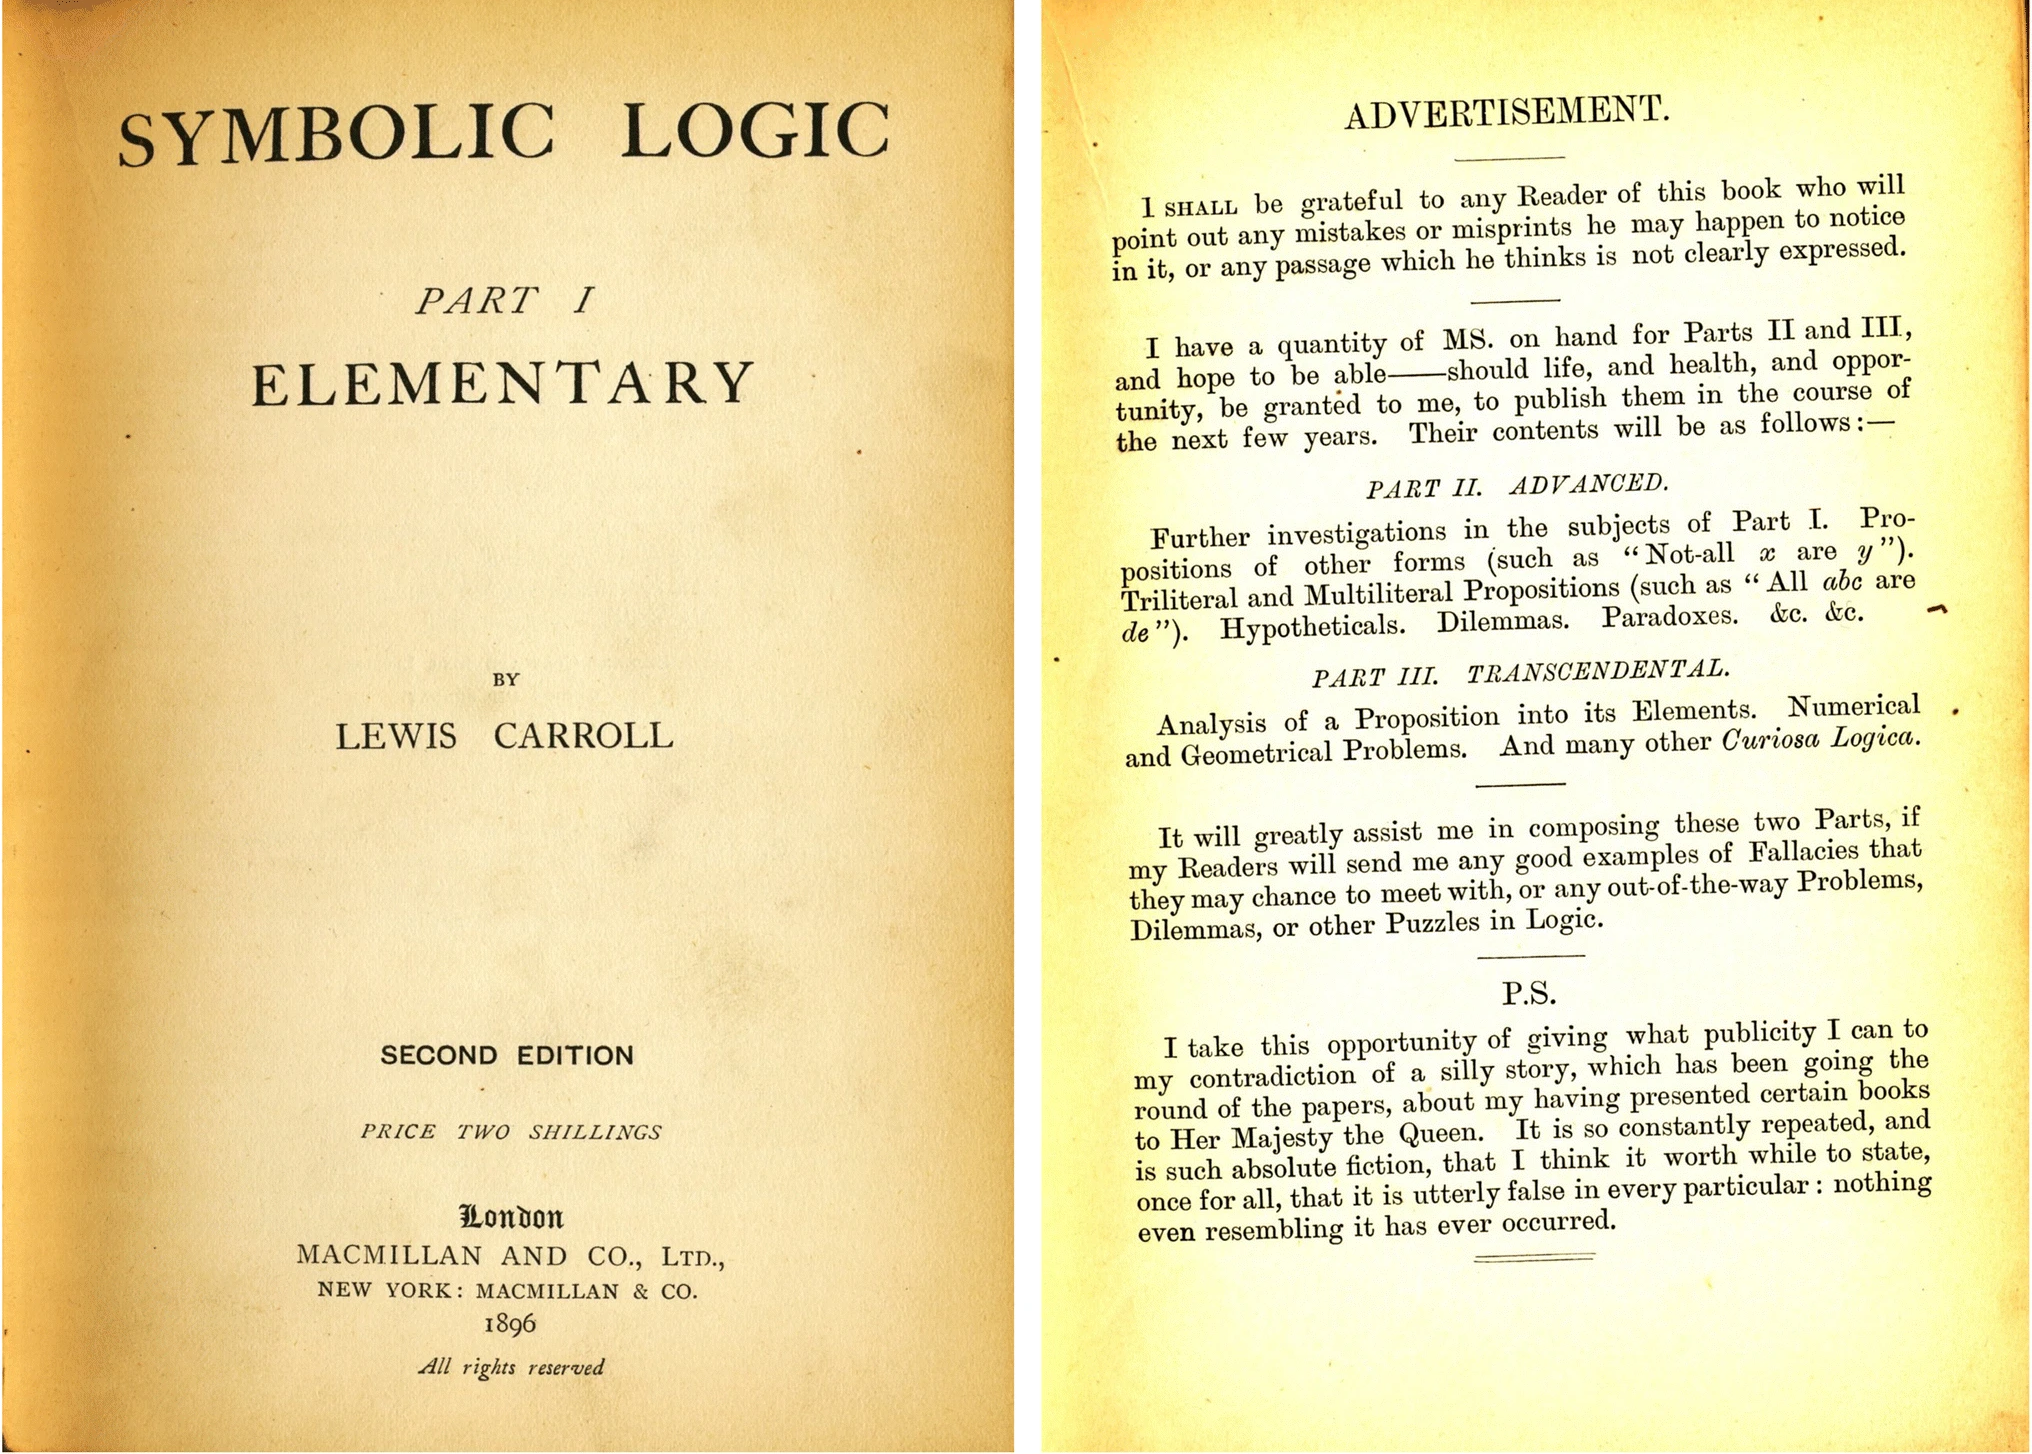
\includegraphics{4}  là số $7$. Để viết các số từ $10$ trở lên, người ta dùng thêm ký hiệu \includegraphics[scale=0.85]{5} (để biểu diễn số $10$), chẳng hạn số $17$ được viết là \includegraphics[scale=0.85]{5}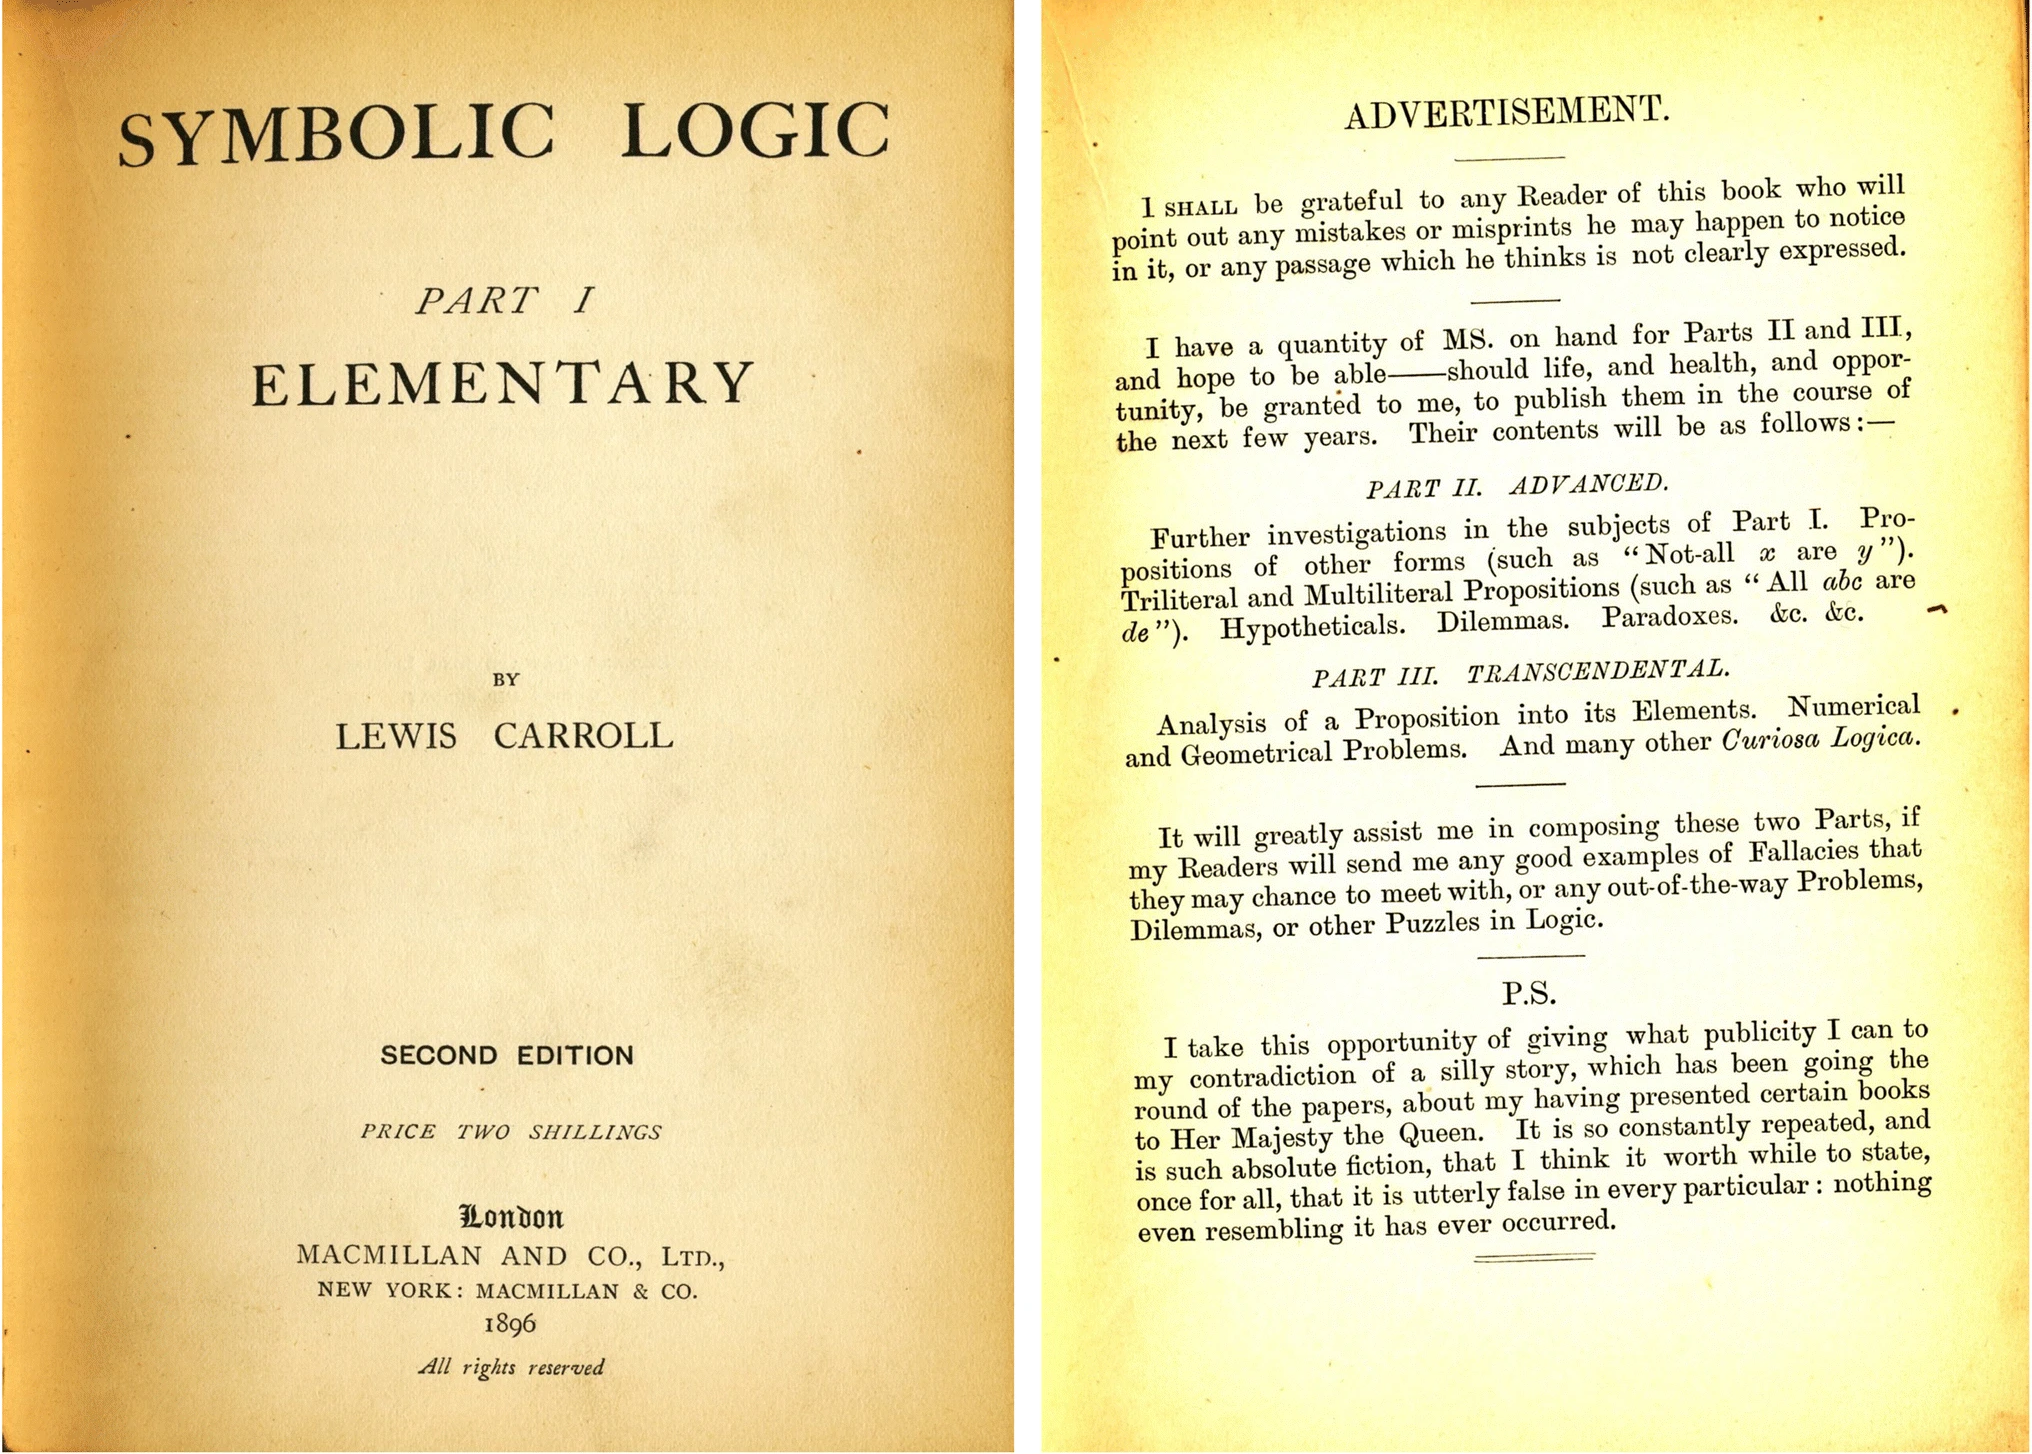
\includegraphics[scale=0.85]{4} và số $27$ được viết là  \includegraphics[scale=0.85]{5}\includegraphics[scale=0.85]{5}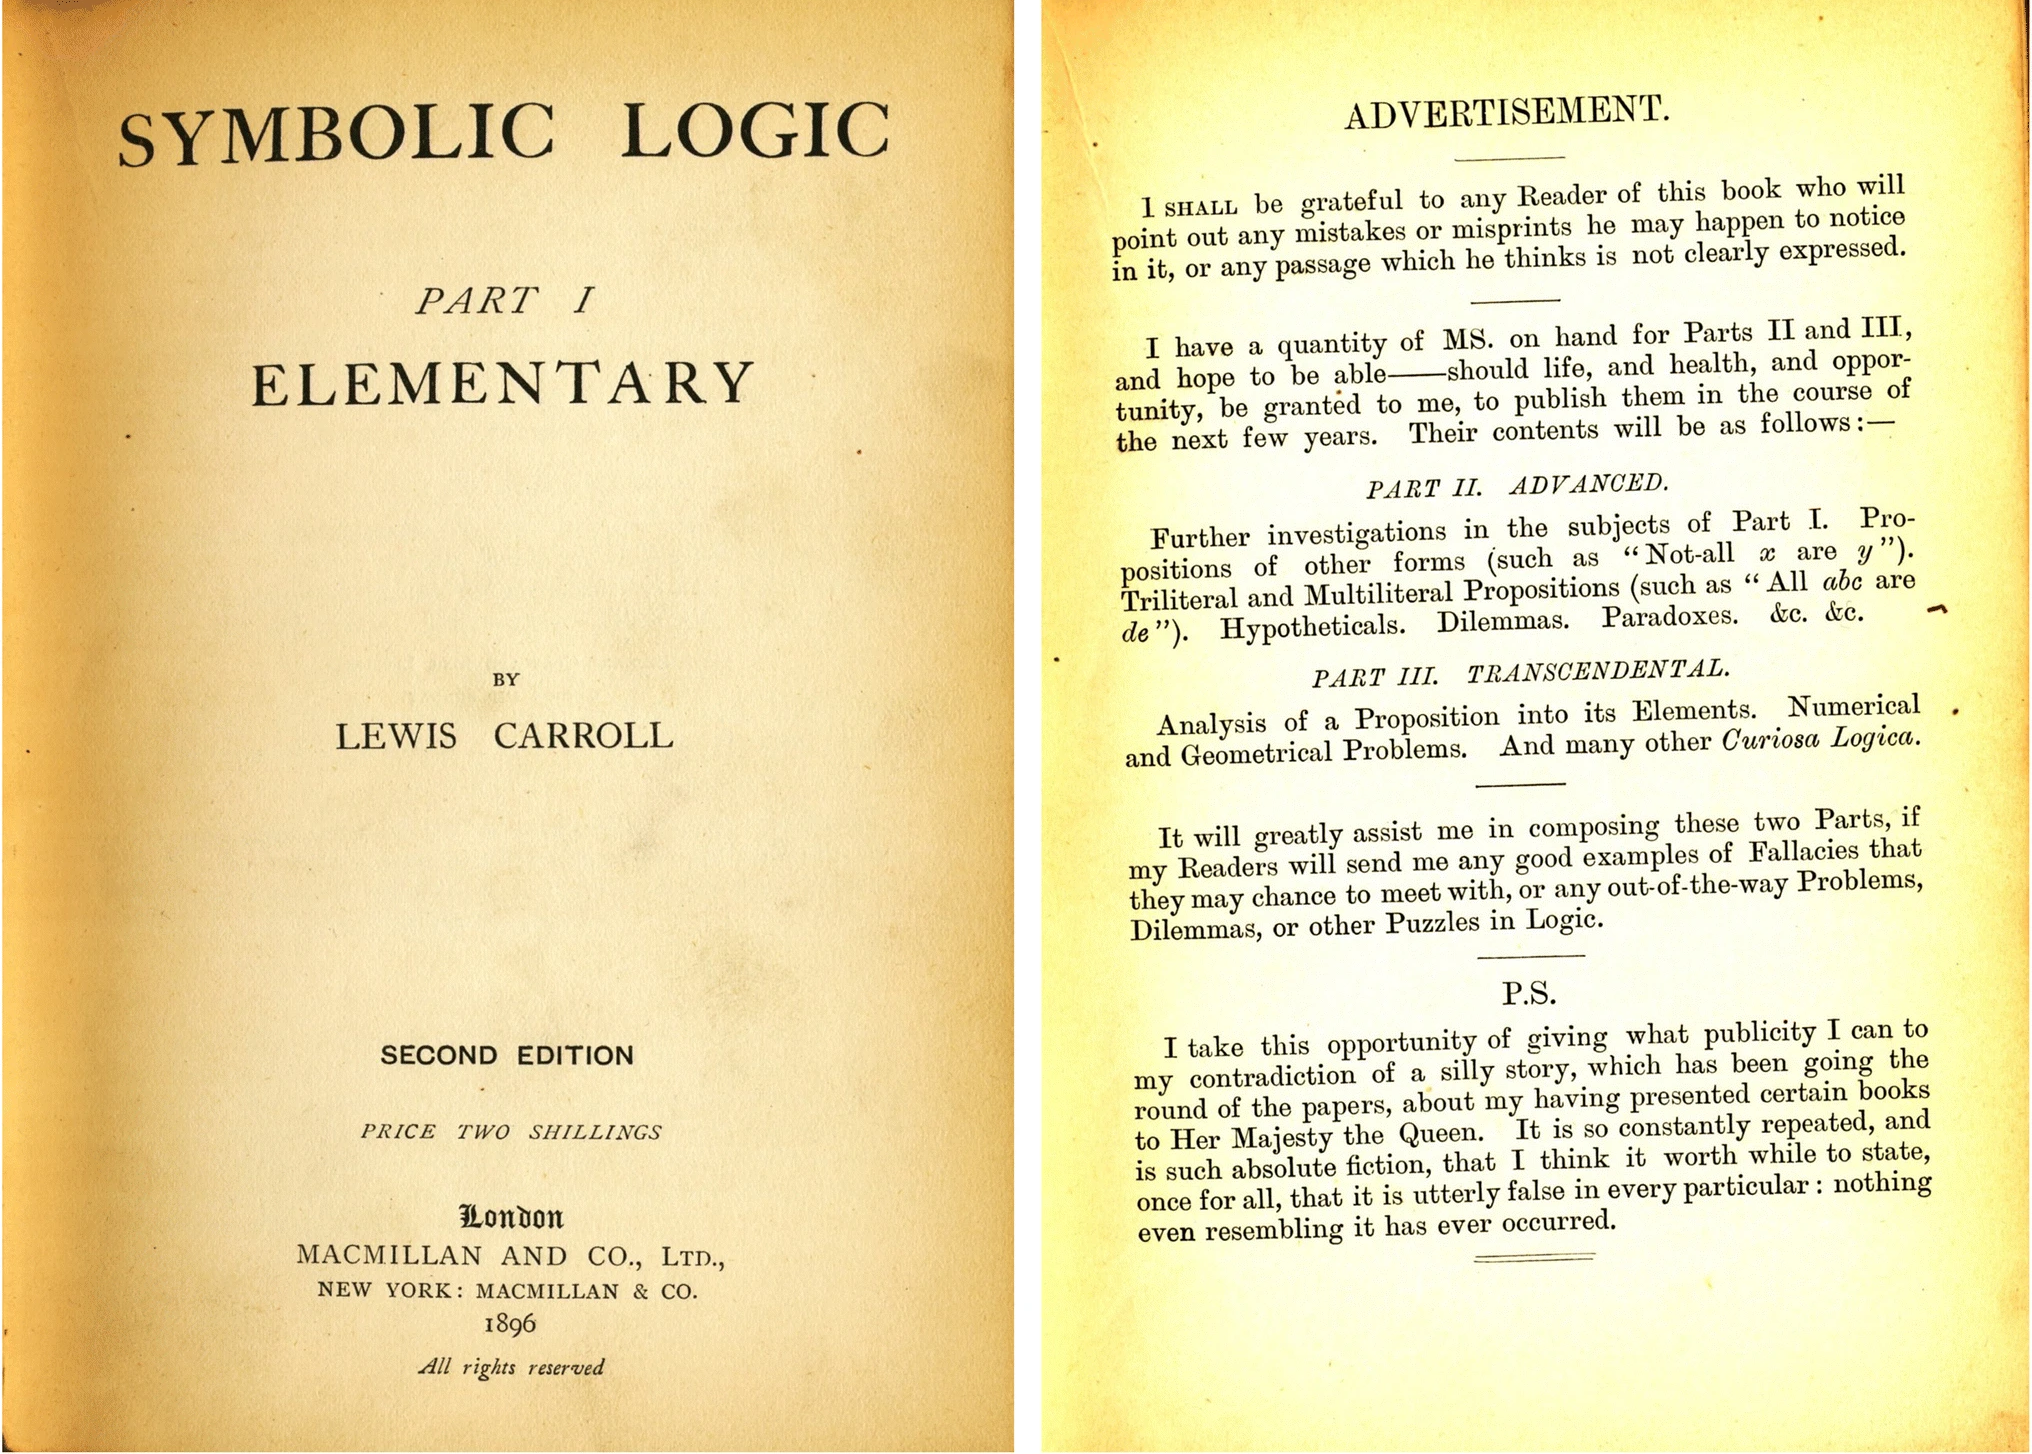
\includegraphics[scale=0.85]{4}. Số lượng các ký hiệu \includegraphics[scale=0.85]{5} cho biết có bao nhiêu chục, số các ký hiệu \includegraphics[scale=1]{12} cho biết có bao nhiêu đơn vị trong số được biểu diễn. Với những số từ $100$ trở đi họ dùng ký hiệu \includegraphics[scale=0.85]{6} (biểu diễn số $100$) và viết các số theo cách tương tự; và cứ như vậy cho những số lớn hơn. Để biết giá trị của số được biểu diễn ta cộng các giá trị ứng với những ký hiệu biểu diễn nó. Chẳng hạn, \includegraphics[scale=0.85]{6}\includegraphics[scale=0.85]{6}\includegraphics[scale=0.85]{5}\includegraphics[scale=0.85]{5}\includegraphics[scale=0.85]{5}\includegraphics[scale=0.85]{3.1}   $=  100+ 100 + 10 + 10 + 10 + 1 + 1 + 1= 233$.
%	\vskip 0.1cm
%	\begin{figure}[H]
%		\centering
%		\vspace*{-5pt}
%		\captionsetup{labelformat= empty, justification=centering}
%		\includegraphics[width=0.7\linewidth]{20.12-pi.1}
%		\vspace*{-10pt}
%	\end{figure}
%	Ngày nay, ta dùng các hàng khác nhau để biểu diễn số: hàng đơn vị, hàng chục, hàng trăm,... Hàng chục đứng ngay trước hàng đơn vị và lớn gấp $10$ lần hàng đơn vị, hàng trăm đứng ngay trước hàng chục và lớn gấp $10$ lần hàng chục,... Đó là cách ghi số trong hệ ``cơ số $10$" hay ``\textit{thập phân}". Cách ghi số của người Ai Cập cổ cũng vậy nhưng việc viết các số phức tạp hơn so với cách viết ngày nay của chúng ta, nhất là với những số lớn. Chẳng hạn để viết số $5412314$, người Ai Cập cổ cần dùng $20$ ký hiệu!
%	\begin{center}
%		$5412314   =$ \includegraphics[scale=0.85]{7}\includegraphics[scale=0.85]{7}\includegraphics[scale=0.85]{7}\includegraphics[scale=0.85]{7}\includegraphics[scale=0.85]{7}\includegraphics[scale=0.35]{fog.png}\includegraphics[scale=0.35]{fog.png}\includegraphics[scale=0.35]{fog.png}\includegraphics[scale=0.35]{fog.png}\includegraphics[scale=0.85]{9}\includegraphics[scale=0.85]{10}\includegraphics[scale=0.85]{10}\includegraphics[scale=0.85]{6}\includegraphics[scale=0.85]{6}\includegraphics[scale=0.85]{6}\includegraphics[scale=0.85]{5}\includegraphics[scale=0.85]{3}
%	\end{center}
%	\vskip 0.1cm
%	\textbf{\color{toancuabi}Số La Mã}
%	\vskip 0.1cm
%	Các bạn có nhìn thấy các ký hiệu I, II, ..., X trên mặt đồng hồ, trong sách vở, trên bảng khi thầy cô giáo đánh số các mục trong bài giảng? Đó là các số La Mã. La Mã là tên gọi một đế chế cổ đại thuộc châu Âu mà có thời kỳ từng thống trị một vùng đất rộng lớn của châu lục này. Người La Mã sử dụng một số chữ cái từ bảng chữ cái của họ để biểu diễn những chữ số.
%	\vskip 0.1cm
%	Số $4$ được viết là IV, còn số $6$ là VI. Khi một chữ số lớn được viết ngay trước  một chữ số nhỏ hơn hay bằng nó, ta cộng chúng lại với nhau để được con số cần biểu diễn, như trường hợp số $6=$ VI. Ngược lại, ta thực hiện phép trừ, giống như trường hợp số $4=$ IV.
%	\begin{table}[H]
%%		\vspace*{-5pt}
%		\centering
%		\setlength{\tabcolsep}{4.5pt}
%		\renewcommand{\arraystretch}{1.25}
%		\begin{tabular}{|l l|l l|}
%			\hline
%			IV $=4$:&    V$-$I $=$ IV & VI $=6$:&    V$+$I =VI\\
%			&$5-1=4$ & &$5+1=6$\\
%			\hline
%		\end{tabular}
%		\vspace*{-10pt}
%	\end{table}
%	Tương tự, ta có:
%	\begin{table}[H]
%		\vspace*{-10pt}
%		\centering
%		\setlength{\tabcolsep}{3.7pt}
%		\renewcommand{\arraystretch}{1.25}
%		\begin{tabular}{|l l|}
%				\hline
%				XXXII $\!=\! 32$:&    X$+$X$+$X$+$I$+$I $\!=\!$ XXXII\\
%				&$10 +10 +10+1+1=32$\\
%				\hline
%				XL$= 40$:&     L $-$ X = XL\\
%				&$50 - 10 = 40$\\
%				\hline
%		\end{tabular}
%	\end{table}
%	\end{multicols}
%	\begin{figure}[H]
%		\centering
%%		\vspace*{-5pt}
%		\captionsetup{labelformat= empty, justification=centering}
%		\includegraphics[width=1\linewidth]{14a}
%		\caption{\small\textit{\color{toancuabi}Các chữ cái và chữ số La Mã}}
%		\vspace*{-10pt}
%	\end{figure}
%	\begin{multicols}{2}
%	Theo cách người La Mã viết số, khi một chữ số nhỏ đứng trước chữ số số lớn hơn, ta trừ số lớn cho số bé. Trong đó I, V chỉ được trừ từ những giá trị không quá X. Ví dụ, ta có thể viết IX nhưng không thể viết IL; X, L chỉ được trừ bởi những chữ số không vượt quá C; C, D chỉ được trừ cho những chữ số không vượt quá M. Ngoài ra, còn có những quy tắc khác như sau:
%	\vskip 0.1cm
%	-- Luôn viết số bằng cách dùng ít ký hiệu nhất, chẳng hạn ta viết XX để biểu diễn $20$ thay vì VVVV.
%	\vskip 0.1cm
%	-- Không có nhiều hơn $3$ ký tự giống nhau trong một hàng (đơn vị, chục, trăm,...). Ví dụ ta viết XIV thay vì XIIII để biểu diễn $14$.
%	\vskip 0.1cm
%	-- Để biểu diễn số gấp hơn $1000$ lần, người La Mã dùng vạch ngang phía trên các dãy chữ số, ví dụ $\overline{\text{VI}}\text{II}=6\times 1000+2=6002$. Ở đây, VI có thêm vạch ngang trên đầu biểu diễn giá trị $6\times 1000 = 6000$. Những chữ số có vạch ngang trên đầu đứng trước các chữ số còn lại.
%	\vskip 0.1cm
%	-- Không đặt nhiều hơn $1$ số nhỏ đứng trước $1$ số lớn. Ví dụ ta không viết IIX để biểu diễn~$8$.
%	\vskip 0.1cm
%	Để dễ dàng viết số La Mã, ta viết theo từng hàng từ  lớn đến nhỏ (như các số mà ngày nay chúng ta dùng). Ví dụ, để viết số $645$, ta viết $600$ trước (DC), rồi $40$ (XL) và cuối cùng là $5$ (V). Vậy $\text{DCXLV}=645$.
%	Số La Mã là hệ số cổ duy nhất còn được dùng ngày nay nhưng cũng chỉ mang ý nghĩa tượng trưng hay để trang trí.
%	\vskip 0.1cm
%	Trong phần hai của bài viết này chúng ta sẽ cùng tìm hiểu  cách ghi số của người Babylon, Maya và Trung Hoa cổ đại. Mời các em đón đọc ở số báo sau. Còn bây giờ chúng ta cùng làm một số bài tập nhé.
%	\vskip 0.1cm
%	\textbf{\color{toancuabi}Bài tập} $\pmb{1.}$ Viết các số sau theo cách viết số ngày nay
%	\vskip 0.1cm
%	$\bullet$ \includegraphics{5}\includegraphics{5}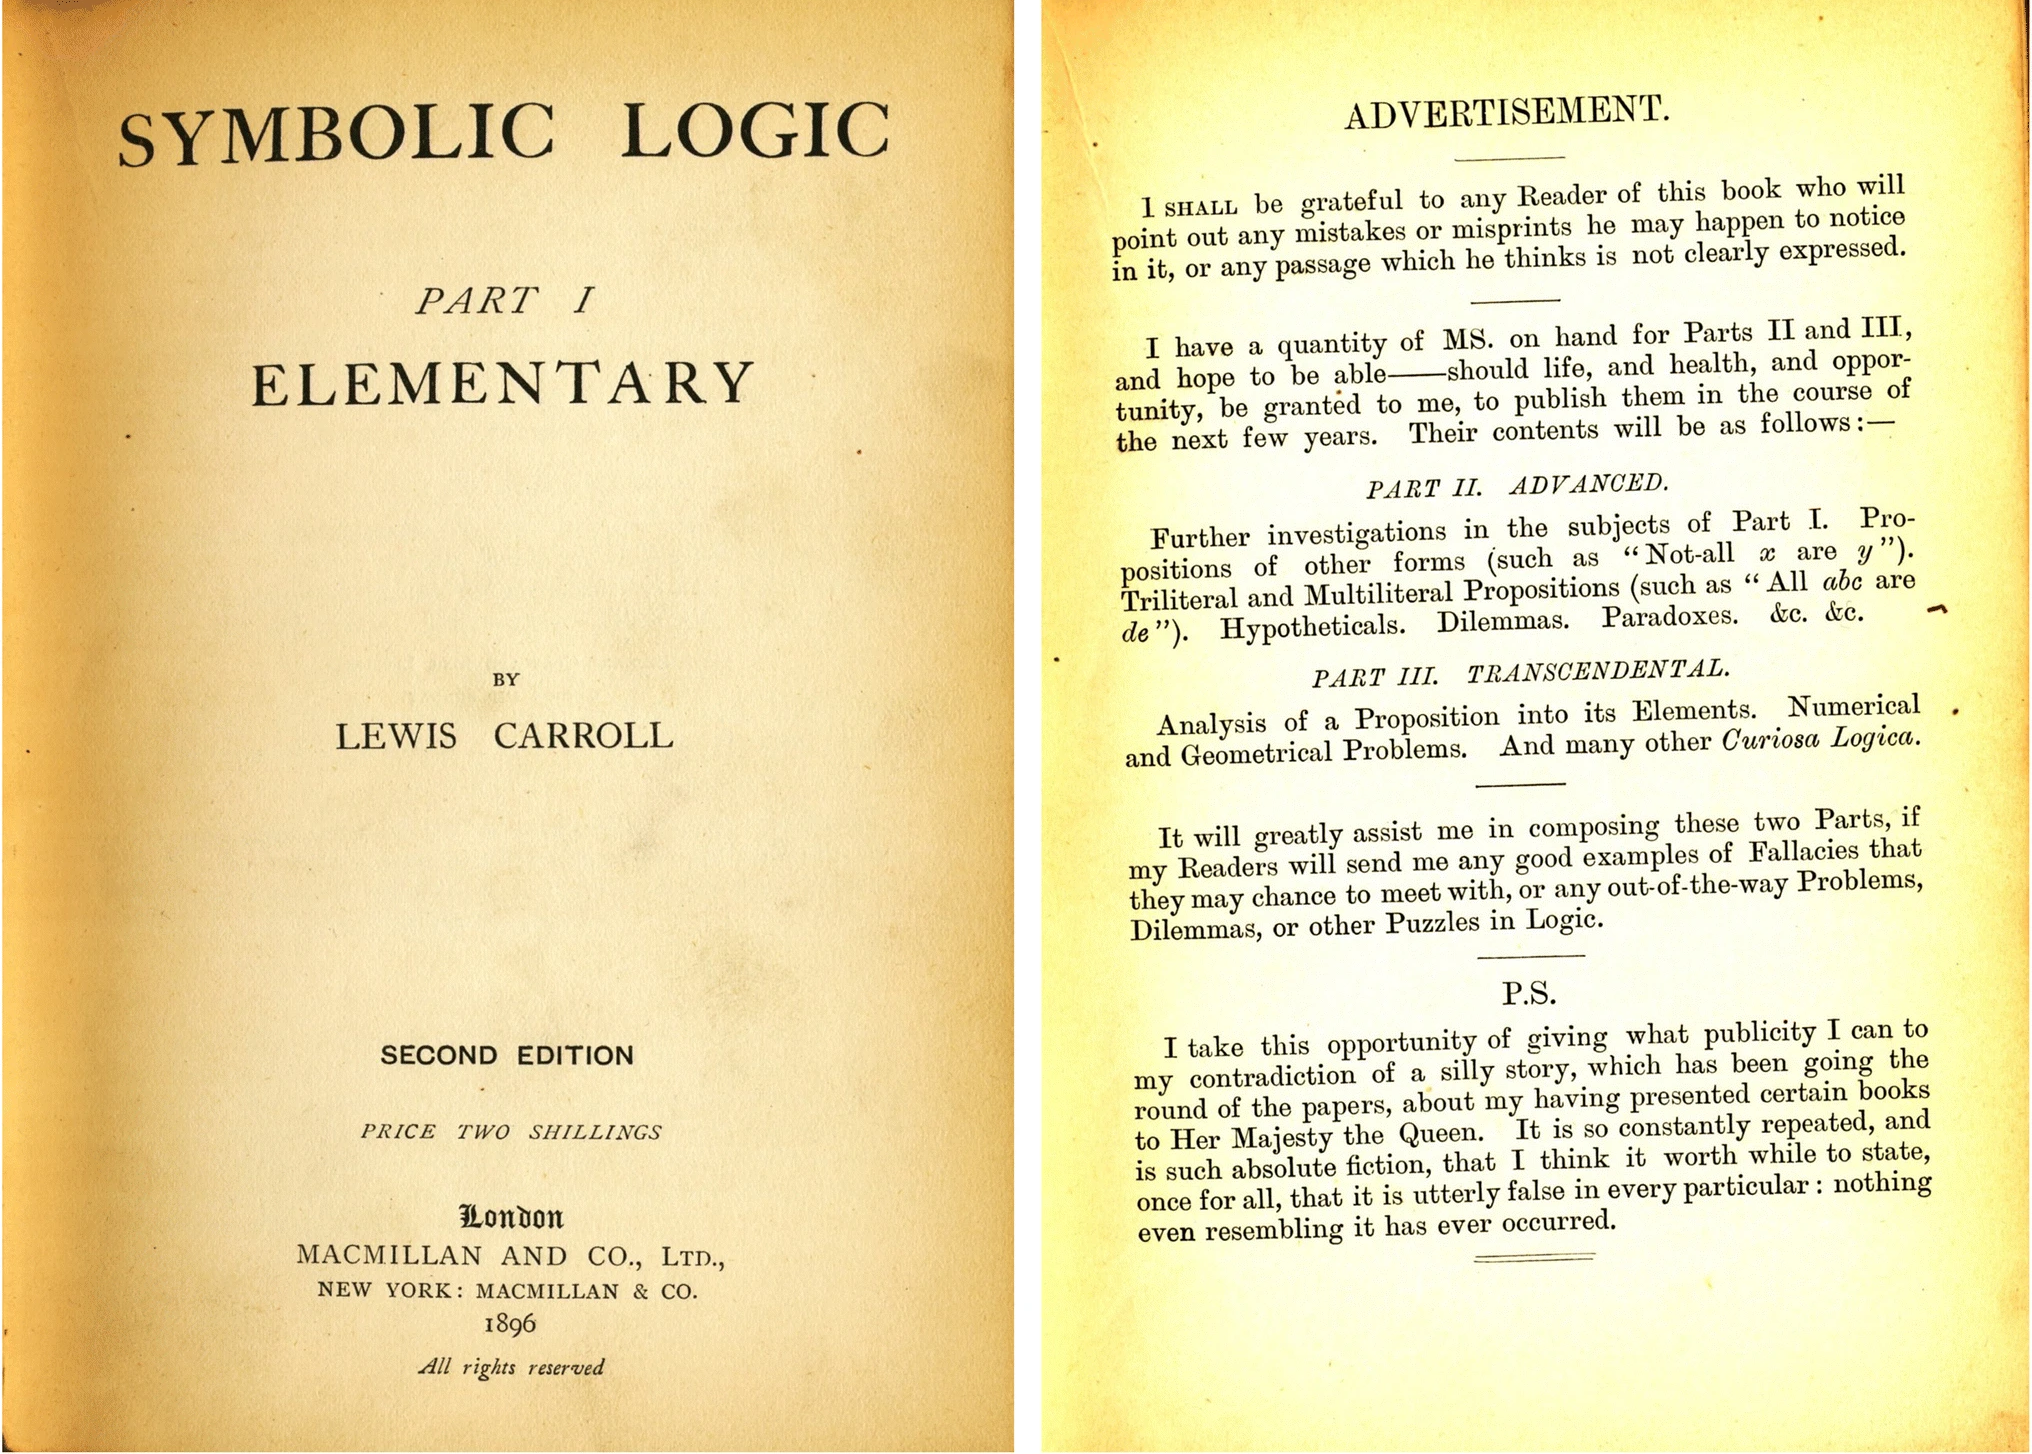
\includegraphics{4}
%	\vskip 0.1cm $\bullet$ \includegraphics{10}\includegraphics{10}\includegraphics{6}\includegraphics{6}\includegraphics{6}
%	\vskip 0.1cm $\bullet$ \includegraphics{9}\includegraphics{10}\includegraphics{10}\includegraphics{6}\includegraphics{3}
%	\vskip 0.1cm
%	$\bullet$ IX
%	\vskip 0.1cm
%	$\bullet$ CLII
%	\vskip 0.1cm
%	$\bullet$ MCCXXX
%	\vskip 0.1cm
%	\textbf{\color{toancuabi}Bài tập} $\pmb{2.}$ Viết các số sau bằng số Ai Cập cổ và số La Mã
%	\vskip 0.1cm
%	$\bullet$ $8$
%	\vskip 0.1cm
%	$\bullet$ $15$
%	\vskip 0.1cm
%	$\bullet$ $999$

	\textbf{\color{toancuabi}Số Babylon}
	\vskip 0.1cm
	Người Babylon, sống vào khoảng $5000$ năm trước ở vùng đất Lưỡng Hà (một khu vực ở phía Tây của  Châu Á). Họ đã tạo ra những công cụ tính toán thiên văn, hình học đáng kinh ngạc và họ đã phát minh ra bàn tính.
		\begin{figure}[H]
		\centering
		\vspace*{-5pt}
		\captionsetup{labelformat= empty, justification=centering}
		\includegraphics[width=1\linewidth]{17.1}
		\vspace*{-15pt}
	\end{figure}
	Để ghi số, ban đầu người Babylon chỉ sử dụng hai ký hiệu 
	\begin{table}[H]
		\vspace*{-10pt}
		\centering
		\begin{tabular}{|c|c|}
			\hline
			& \\[-2.5ex]
			\includegraphics[scale=0.7]{15}&$1$\\
			\hline
			& \\[-2.5ex]
			\includegraphics[scale=0.65]{16}&$10$\\
			\hline
		\end{tabular}
		\vspace*{-10pt}
	\end{table}
	để viết số từ $1$ tới $60$, chẳng hạn số $7$ là  \includegraphics[scale=0.7]{17}, số $27$ là  \includegraphics[scale=0.7]{16}\includegraphics[scale=0.7]{16}\includegraphics[scale=0.7]{17}. 	 
	\vskip 0.1cm
	Những ký hiệu này được sử dụng tương tự như những chữ số La Mã (bằng cách cộng các ký hiệu xuất hiện trong số được biểu diễn). Số \includegraphics[scale=0.7]{18} được viết bởi $2$ ký hiệu \includegraphics[scale=0.7]{16} để biểu diễn $2$ chục, và $7$ ký hiệu \includegraphics[scale=0.7]{15}  cho $7$ đơn vị. Do vậy \includegraphics[scale=0.7]{18}  $=27$.
	\vskip 0.1cm
	Sau đó, một ký hiệu mới được sử dụng để biểu diễn chữ số $0$ (các bạn có thấy nó là ký tự chỉ chữ số $1$ được viết ngiêng?)
	\includegraphics[scale=0.65]{15.1}
	\vskip 0.1cm
	Để viết những số từ $60$ trở đi, người Babylon xếp các ký hiệu theo các nhóm. Điều này giống như ngày nay các bạn viết $159$ bằng cách viết số $1$ đầu tiên ứng với hàng trăm, số $5$ tiếp theo ở hàng chục và cuối cùng là số $9$ ở hàng đơn vị. Như vậy $159 = 1 \times 100+ 5 \times 10+ 9$.
	\vskip 0.1cm
	\begin{figure}[H]
		\centering
		\vspace*{-5pt}
		\captionsetup{labelformat= empty, justification=centering}
		\includegraphics[width=0.85\linewidth]{20.12-pi.2}
		\vspace*{-15pt}
	\end{figure}
	Để viết số $63$, người Babylon viết ký hiệu  \includegraphics[scale=0.7]{15}  ở hàng $60$ và ba ký hiệu \includegraphics[scale=0.7]{15}  ở hàng đơn vị và để khoảng trống để phân biệt hai nhóm.
	\vskip 0.1cm
	\includegraphics[scale=0.7]{16.1}$=63$. Trong cách viết này, ta thấy có $4$ ký hiệu \includegraphics[scale=0.7]{15}   nhưng ký hiệu đầu tiên được viết tách biệt so với $3$ cái còn lại để biểu diễn $1$ lần $60$ tức $60$, $3$ ký hiệu còn lại biểu diễn số $3$, và như vậy ta có số $60+3 =63$.
	\vskip 0.1cm
	Điều này giống như chúng ta viết chữ số $1$ ở hàng chục và chữ số $1$ ở hàng đơn vị để biểu diễn số $11$: nó có nghĩa là $1$ chục và $1$ đơn vị. Trong  cách ghi số  Babylon cổ, nó có nghĩa là $1$ lần $60$  và $1$.
	\vskip 0.1cm
	Để hiểu rõ hơn, ta hãy viết số chín mươi ba theo hệ ghi số hiện đại. Việc này thật dễ dàng phải không? Tuy nhiên để hiểu cách viết của người Babylon, ta sẽ thực hiện theo cách như sau: do các số của chúng ta ngày nay sử dụng hệ cơ số $10$, ta chia chín mươi ba cho $10$ được thương là $9$, nên ta viết $9$ vào hàng chục
	\begin{figure}[H]
		\centering
		\vspace*{-5pt}
		\captionsetup{labelformat= empty, justification=centering}
		\includegraphics[width=0.65\linewidth]{19}
		\vspace*{-10pt}
	\end{figure}
	Phép chia đó có số dư $3$ nên ta viết $3$ vào hàng đơn vị
	\begin{figure}[H]
		\centering
		\vspace*{-5pt}
		\captionsetup{labelformat= empty, justification=centering}
		\includegraphics[width=0.65\linewidth]{20}
		\vspace*{-10pt}
	\end{figure}
	Vậy là ta viết: $93$.
	\vskip 0.1cm
	Thế còn người Babylon viết số $93$ trong hệ thống số của họ như thế nào?
	\vskip 0.1cm
	\textit{Hệ thống số Babylon sử dụng hệ cơ số $60$}: ta chia $93$ cho $60$ được thương là $1$ nên ta viết $1$ ở hàng $60$
	\begin{figure}[H]
		\centering
		\vspace*{-5pt}
		\captionsetup{labelformat= empty, justification=centering}
		\includegraphics[width=0.65\linewidth]{21}
		\vspace*{-10pt}
	\end{figure}
	Phép chia có số dư là $33$, nên ta sẽ viết $33$ ở hàng đơn vị. Số $33$ được biểu diễn bởi $3$ ký tự mười cộng với $3$. Nên ta đặt $3$ ký tự \includegraphics[scale=0.65]{16} và $3$ ký tự \includegraphics[scale=0.65]{15} vào hàng đơn vị như sau
	\begin{figure}[H]
		\centering
		\vspace*{-5pt}
		\captionsetup{labelformat= empty, justification=centering}
		\includegraphics[width=0.65\linewidth]{22}
		\vspace*{-10pt}
	\end{figure}
	Vậy \includegraphics[scale=0.85]{23}  $= 93$.
	\vskip 0.1cm
	Tiếp theo, chúng ta hãy thử viết số lớn hơn. Chúng ta hãy cùng viết số $3604$ bằng các chữ số Babylon nhé. Số $3604$ lớn hơn $60\times 60=3600$, nên ta cần biểu diễn số này từ hàng thứ ba tính từ hàng đơn vị. Ta chia số $3604$ cho $3600$ được thương là $1$ nên ta viết ký hiệu \includegraphics[scale=0.7]{15}  vào hàng $60\times60$
	\begin{figure}[H]
		\centering
		\vspace*{-5pt}
		\captionsetup{labelformat= empty, justification=centering}
		\includegraphics[width=0.65\linewidth]{25}
		%	\caption{\textit{\color{toancuabi}Hình $1$.}}
		\vspace*{-10pt}
	\end{figure}
	Số dư của phép chia là $4$ nhỏ hơn $60$ nên ta viết ký hiệu \includegraphics[scale=0.6]{15.1} vào hàng $60$, và $4$ ký hiệu \includegraphics[scale=0.7]{15} vào hàng đơn vị. 
	\begin{figure}[H]
		\centering
		\vspace*{-5pt}
		\captionsetup{labelformat= empty, justification=centering}
		\includegraphics[width=0.65\linewidth]{26}
		%	\caption{\textit{\color{toancuabi}Hình $1$.}}
		\vspace*{-10pt}
	\end{figure}
	Vậy, số $3604$ được người Babylon viết như sau:
	\begin{figure}[H]
		\centering
%		\vspace*{-5pt}
		\captionsetup{labelformat= empty, justification=centering}
		\includegraphics[width=0.75\linewidth]{27}
		%	\caption{\textit{\color{toancuabi}Hình $1$.}}
		\vspace*{-10pt}
	\end{figure}
	Cách ghi Số của người Ai Cập cổ, La Mã hay chúng ta ngày nay dùng cơ số $10$ còn cách ghi số của người Babylon sử dụng cơ số $60$. Do số $60$ chia hết cho nhiều số: $1,2,3,4,5,6, 10, 12, 15, 20,30$ và $60$, nên việc chia các đại lượng được thực hiện dễ dàng hơn, ít phải dùng đến các phân số. Việc sử dụng đơn vị thời gian: $1$ phút $= 60$ giây, $1$ giờ $= 60$ phút ngày nay là một ảnh hưởng của người Babylon đấy.
	\vskip 0.1cm
	\textbf{\color{toancuabi}Số Maya}
	\vskip 0.1cm
	\begin{figure}[H]
		\centering
		\vspace*{-10pt}
		\captionsetup{labelformat= empty, justification=centering}
		\includegraphics[width=1\linewidth]{28}
		\caption{\textit{\color{toancuabi}Kim tự tháp Tikal của người Maya}}
		\vspace*{-15pt}
	\end{figure}
	Người Maya  được cho là đã xuất hiện từ rất xa xưa. Họ đã xây dựng hệ thống lịch chính xác và toán học của họ là đại diện tiêu biểu cho toán học của dân cư ở châu Mỹ thời cổ đại.
	\vskip 0.1cm
	Nói về cách ghi số,  người Maya  cổ dùng hệ cơ số $20$, gồm $3$ ký hiệu:  \includegraphics[scale=0.7]{29},  \includegraphics[scale=0.7]{30}, \includegraphics[scale=0.7]{31}  ứng với $0,1, 5$ và biểu diễn số theo chiều dọc. Chữ số ở hàng cao hơn được viết phía trên, chữ số ở hàng thấp hơn được viết phía dưới. Điều này tương tự chúng ta viết số ngày nay: ta đặt số ở hàng cao hơn bên trái còn số ở hàng thấp hơn bên phải. 
	\begin{table}[H]
		\vspace*{-5pt}
		\centering
		\setlength{\tabcolsep}{4.5pt}
		\renewcommand{\arraystretch}{1.25}
		\begin{tabular}{|l|l|}
			\hline
			$10^3 = 10\!\times\! 10 \!\times\! 10 =1000$& hàng nghìn\\
			\hline
			$10^2 = 10\!\times\! 10 =100$& hàng trăm\\
			\hline
			$10^1 = 10$& hàng chục\\
			\hline
			$10^0 = 1$& hàng đơn vị\\
			\hline
		\end{tabular}
%		\vspace*{-5pt}
	\end{table}
	Do sử dụng hệ cơ số $20$,  số Maya được biểu diễn trong phần bên phải của bảng trong Hình $3$ chính là số  $1\times 8000+ 0\times 400+ 10\times20+ 7\times1= 8207$. Bởi vì, ta  thấy  \includegraphics[scale=0.3]{33},  \includegraphics[scale=0.3]{34},  \includegraphics[scale=0.3]{35}, \includegraphics[scale=0.3]{36}  ứng với $1, 0, 10, 7$  lần lượt ở các hàng $8000$, $400$, $20$ và đơn vị. Chú ý rằng, trong một hàng, số có giá trị cao hơn lại được viết phía dưới số có giá trị lớn hơn chẳng hạn  \includegraphics[scale=0.3]{36}:  hai ký tự \includegraphics[scale=0.7]{37} (số $1$) được viết bên trên ký tự \includegraphics[scale=0.7]{38} (số $5$). Ký hiệu \includegraphics[scale=0.3]{34} để biểu diễn $0$ ở một hàng giống như ta viết $101$ và giúp ta phân biệt số $101$ với số $11$. Điều này cũng tương tự như cách ghi số Babylon. 
	\begin{table}[H]
		\vspace*{-5pt}
		\centering
		\captionsetup{labelformat= empty, justification=centering}
		\setlength{\tabcolsep}{21pt}
		\renewcommand{\arraystretch}{1.25}
		\begin{tabular}{|l|c|}
			\hline
			$20\times 20\times 20 =8000$  & \includegraphics[scale=0.3]{33} \\
			\hline
			$20\times 20 =400$     & \includegraphics[scale=0.3]{34} \\
			\hline
			$20$ & \includegraphics[scale=0.3]{35}\\
			\hline
			$1$& \includegraphics[scale=0.3]{36.png}\\
			\hline
		\end{tabular}
		\caption{\small\textit{\color{toancuabi}Hình $3$.}}
		\vspace*{-10pt}
	\end{table}
	Người ta cho rằng hệ cơ số $10$ được dùng phổ biến vì con người có $10$ ngón tay, còn người Maya vốn không đi giày nên họ đếm bằng cả các ngón chân nữa. Họ dùng hệ cơ số $20$ là vì thế!
	\begin{figure}[H]
		\centering
		\vspace*{-5pt}
		\captionsetup{labelformat= empty, justification=centering}
		\includegraphics[width=1\linewidth]{20.12-pi.4-2}
		\vspace*{-12pt}
	\end{figure}
	\vskip 0.1cm
	\textbf{\color{toancuabi}Số Trung Hoa cổ}
	\vskip 0.1cm
	Trung Hoa cổ đại cũng là một trong những nền văn minh cổ lớn của thế giới. Khoảng $3500$ năm trước, người Trung Hoa khắc lên những mảnh mai rùa những ký hiệu khác nhau thể hiện số và chữ. Một số trong đó như~sau:
	\begin{figure}[H]
		\centering
%		\vspace*{-5pt}
		\captionsetup{labelformat= empty, justification=centering}
		\includegraphics[height=0.45\linewidth]{40}\quad
		\includegraphics[height=0.45\linewidth]{41}
		\caption{\textit{\color{toancuabi}Một số ký hiệu viết trên một mảnh mai rùa.}}
		\vspace*{-10pt}
	\end{figure}
	Cách ghi số Trung Hoa cổ tương tự như cách ghi số La Mã: Các chữ số giá trị lớn được đặt bên trái các chữ số có  giá trị nhỏ hơn, số được biểu diễn có giá trị bằng tổng các chữ số trong biểu diễn của nó. Ví dụ \includegraphics[scale=0.7]{42} biểu diễn số $10000 + 500 + 30 + 5 =10535$. Những biểu tượng khắc trên những mảnh mai rùa phát triển theo thời gian và hình thành nên chữ viết của người Trung Hoa ngày nay. 
	\vskip 0.1cm
	Các bạn có thấy rằng cách biểu diễn số của người Ai Cập, La Mã và Trung Hoa cổ có điểm tương đồng? Người ta nói đó là những hệ thống số ``\textit{đơn phân}". Mỗi ký hiệu thể hiện một giá trị không thay đổi cho dù nó đứng ở vị trí nào. Mỗi số viết ra biểu diễn một đại lượng được xác định bằng cách  cộng (hay trừ như ở số La Mã) những giá trị tương ứng với các ký hiệu được sử dụng trong đó. Số mà chúng ta dùng ngày nay là một hệ thống số ``\textit{sắp theo hàng}" vì các ký hiệu có giá trị phụ thuộc vào hàng mà nó được xếp vào. Ở hàng chục, số $1$ có nghĩa là một chục, nhưng số $1$ ở hàng đơn vị có nghĩa là $1$ đơn vị. Trong khi đó, số của người Babylon và Maya là một dạng hỗn hợp vừa được ``\textit{sắp theo hàng}" vừa cần cộng những ký hiệu trong mỗi hàng để biết giá trị của số được biểu diễn.
	\begin{figure}[H]
		\centering
		\vspace*{-5pt}
		\captionsetup{labelformat= empty, justification=centering}
		\includegraphics[width=0.85\linewidth]{20.12-pi.3}
		\vspace*{-10pt}
	\end{figure}
	Vậy là qua bài viết này chúng ta đã biết những cách ghi số  từ thời xa xưa con người ở những nơi khác nhau trên Trái Đất. Những đại lượng phức tạp hơn như phân số chẳng hạn cũng đã được người cổ đại viết ra và sử dụng. Chúng ta sẽ tìm hiểu thêm về những thành tựu toán học của loài người ở những thời kỳ trước đây trong những số báo sắp tới nhé. 
	\vskip 0.1cm
	\textbf{\color{toancuabi}Tài liệu, nguồn tham khảo}
	\vskip 0.1cm
	[$1$] R. L. Cooke, History of math, Wiley, $2013$.
	\vskip 0.1cm
	[$2$] \url{https://www.britannica.com/}
	\vskip 0.1cm
	[$3$] \url{https://www.penn.museum/}
	\vskip 0.1cm
	[$4$] \url{https://www.cemc.uwaterloo.ca}
\end{multicols}
%\newpage
%\graphicspath{{../toancuabi/pic/}}
%\begingroup
%\AddToShipoutPicture*{\put(112,680){\includegraphics[scale=1]{../tieude.pdf}}} 
%\centering
%\endgroup
%\vspace*{25pt}
%
%\begin{multicols}{2}
%	Một lần nọ, thám tử Xuân Phong lên đường để truy tìm một kẻ tội phạm có biệt hiệu là Bắp Cải đang lẩn trốn trong một khu lán trại hẻo lánh có tên là Vườn Ngô. Xuân Phong vừa đi vừa hỏi đường vì bản đồ không chỉ rõ khu Vườn Ngô ở đâu, chắc hẳn đó là một địa điểm mới trong vùng. Thám tử đang lơ ngơ tìm đường thì bỗng nhiên một bác nông dân vui tính, tay cầm cuốc, mồ hôi nhễ nhại, xuất hiện trước mặt. Bác hồ hởi vừa nói vừa đưa tay ra hiệu: ``Tôi biết đường đến khu Vườn Ngô chứ, tôi đã từng đến đó rồi. Lần đó, tôi đi mất  tận $4$ ngày và $4$ đêm. Ngày và đêm đầu tiên tôi đi trên đường cái thẳng về phía bắc, và đi được một phần ba quãng đường. Sau đó tôi quay về phía tây và gắng sức đi xuyên qua rừng mất một ngày một đêm nữa, và đi được quãng đường chỉ bằng nửa của ngày đêm đầu tiên. Ngày và đêm thứ ba tôi lại phải đi xuyên qua rừng tiếp, và đi về phía nam và cuối cùng lại đi ra đường cái dẫn về phía đông. Tôi đi rảo bước theo con đường đó cả ngày cả đêm thứ tư, đi hết $30$ km và thế là đặt chân đến được khu Vườn Ngô, nơi mà thám tử đang tìm. Đấy, thám tử cứ đi theo con đường sáng suốt như tôi đã đi là thế nào sang tới ngày thứ $5$ sẽ tới được Vườn Ngô".
%	\vskip 0.1cm
%	Xuân Phong suy nghĩ một chút rồi xua tay trả lời ``Cảm ơn bác nhé. Nếu mọi thứ cứ đúng như bác nói thì ngay ngày mai tôi đã có thể đặt chân tới Vườn Ngô và bắt được tên Bắp~Cải."
%	\begin{figure}[H]
%		\centering
%		\vspace*{-5pt}
%		\captionsetup{labelformat= empty, justification=centering}
%		\includegraphics[width=1\linewidth]{xp}
%		\vspace*{-15pt}
%	\end{figure}
%	Xuân Phong có lập luận đúng không nhỉ? Theo em, bác nông dân đã đi bao nhiêu km để tới Vườn Ngô, còn Xuân Phong thì nghĩ sẽ cần phải đi hết bao nhiêu km?
%\end{multicols}
%\vspace*{-10pt}
%\rule{1\linewidth}{0.1pt}
%\begingroup
%\AddToShipoutPicture*{\put(112,248){\includegraphics[scale=1]{../tieude11.pdf}}} 
%\centering
%\endgroup
%\vspace*{40pt}
%
%\begin{multicols}{2}
%	$\pmb{1.}$ Một lần nọ, sau cơn mưa, bác Tuấn đi vào rừng để hái nấm. Bác khệ nệ bê được cả một sọt nấm nặng trĩu về. Nhưng thật buồn cho bác là về đến nhà, bác mới biết là trong số nấm tươi mới hái được thì có tới tận $90\%$ thành phần là nước, nên hoá ra bác mất công mang nước về suốt cả một quãng đường dài. Sau khi nấm được hong khô đi chút, khối lượng của đống nấm bị giảm đi $15$ kg, và bây giờ nước chỉ chiếm $60\%$ khối lượng. Hỏi lúc đầu bác Tuấn đã mang được bao nhiêu ki--lô--gam nấm từ rừng về nhà?
%	
%	\columnbreak
%	\begin{figure}[H]
%		\centering
%%		\vspace*{5pt}
%		\captionsetup{labelformat= empty, justification=centering}
%		\includegraphics[width=0.65\linewidth]{bai1}
%	\end{figure}
%	\end{multicols}
%	\begin{multicols}{2}
%	$\pmb{2.}$ Ông Ninh cùng với con trai mình và ông Phúc cùng với con trai mình đi ra hồ câu cá. Ông Ninh bắt được số con cá bằng với số con cá mà con trai ông  bắt được. Còn ông Phúc lại bắt được số con cá nhiều gấp ba lần số con cá mà con trai ông bắt được. Họ bắt được tổng cộng  $35$ con. Con trai của ông Ninh đi câu cá cùng ông tên là Giao. Hỏi con ông Phúc tên là gì và mỗi người hôm đó bắt được bao nhiêu con cá?
%	\begin{figure}[H]
%		\centering
%		\vspace*{-5pt}
%		\captionsetup{labelformat= empty, justification=centering}
%		\includegraphics[width=1\linewidth]{bai2}
%		\vspace*{-15pt}
%	\end{figure}
%	$\pmb{3.}$ Chiếc đồng hồ treo tường nhà bạn Lâm chỉ  $9$ giờ $20$ phút. Hỏi lúc đó góc tạo bởi kim giờ và kim phút bằng bao nhiêu độ (góc tương ứng với một vòng tròn là $360$ độ)?
%	\begin{figure}[H]
%		\centering
%		\vspace*{-5pt}
%		\captionsetup{labelformat= empty, justification=centering}
%		\includegraphics[width=1\linewidth]{bai3}
%		\vspace*{-15pt}
%	\end{figure}
%	$\pmb{4.}$ Tích của một tỷ số tự nhiên bằng đúng $1$ tỷ. Hỏi giá trị lớn nhất của tổng của chúng bằng bao nhiêu?
%	\begin{figure}[H]
%		\centering
%		\vspace*{5pt}
%		\captionsetup{labelformat= empty, justification=centering}
%		\includegraphics[width=1\linewidth]{bai5}
%		\vspace*{-15pt}
%	\end{figure}
%	$\pmb{5.}$ Làm thế nào để xác định tâm của một hình tròn nếu chỉ có một cái bút chì và một cái thước kẻ thông thường có hai cạnh song song (chiều rộng của thước kẻ nhỏ hơn đường kính của hình tròn).
%	\begin{figure}[H]
%		\centering
%		\vspace*{-5pt}
%		\captionsetup{labelformat= empty, justification=centering}
%		\includegraphics[width=1\linewidth]{bai4}
%		\vspace*{-15pt}
%	\end{figure}
%	$\pmb{6.}$ Tất cả các điểm của một đường tròn được tô bằng hai màu: trắng hoặc đỏ. Em hãy chứng tỏ rằng luôn có một tam giác cân có các đỉnh nằm trên đường tròn đã cho sao cho các đỉnh của nó đều được tô bởi cùng một màu.
%	\begin{figure}[H]
%		\centering
%		\vspace*{-5pt}
%		\captionsetup{labelformat= empty, justification=centering}
%		\includegraphics[width=1\linewidth]{bai6}
%		\vspace*{-5pt}
%	\end{figure}
%\end{multicols}
%\newpage
%\begingroup
%\AddToShipoutPicture*{\put(112,640){\includegraphics[scale=1]{../tieude2.pdf}}} 
%\centering
%\endgroup
%\graphicspath{{../toancuabi/pic/}}
%\vspace*{70pt}
%
%\begin{multicols}{2}
%	$\pmb{1.}$	Trong một giải thi đấu bóng chuyền, mỗi đội sẽ lần lượt thi đấu với các đội còn lại hai lần. Cuối cùng người ta thấy rằng $80\%$ các đội có ít nhất một trận thắng. Hỏi có tất cả bao nhiêu đội đã tham gia trong giải đấu đó biết rằng các trận đấu bóng chuyền không có tỷ số hoà?
%	\begin{figure}[H]
%		\vspace*{-5pt}
%		\centering
%		\captionsetup{labelformat= empty, justification=centering}
%		\includegraphics[width= 1\linewidth]{b5}
%		\vspace*{-15pt}
%	\end{figure}
%	\textit{Lời giải.} 	Do trong môn bóng chuyền không có trận hoà, nên đội nào không thắng ít nhất một trận có nghĩa là đội đó thua tất cả các đội còn lại. Nhưng chỉ có thể có duy nhất một đội là như vậy, vì không thể có hai đội $A$, $B$ mà $A$ thua $B$ đồng thời $B$ thua $A$ trong cùng trận đấu. Vì thế $20\%$ số các đội bao gồm đúng duy nhất $1$ đội, có nghĩa là  chỉ có đúng $5$ đội tham gia giải đấu đó.
%	\vskip 0.1cm
%	$\pmb{2.}$	Một buổi cắm trại có $9$ học sinh nam và $10$ học sinh nữ tham gia. Trước đó, mỗi học sinh nam đều đã quen với cùng một số lượng các học sinh nữ tham gia buổi cắm trại đó, còn tất cả các học sinh nữ đều quen số lượng học sinh nam hoàn toàn khác nhau (không có hai em nữ nào có số lượng bạn nam quen biết giống nhau). Hỏi điều này có thể xảy ra hay không?
%	\begin{figure}[H]
%		\vspace*{5pt}
%		\centering
%		\captionsetup{labelformat= empty, justification=centering}
%		\includegraphics[width= 1\linewidth]{b4}
%		\vspace*{-15pt}
%	\end{figure}
%	\textit{Lời giải.} 	Giả sử mỗi học sinh nam quen $k$ học sinh nữ, thì khi đó có tất cả $9k$ mối quen biết. Do các bạn nữ có số bạn nam quen biết là hoàn toàn khác nhau, nên điều này chỉ có thể xảy ra nếu một bạn quen với tất cả $9$ bạn nam, một bạn quen với $8$ bạn nam, vv... và cuối cùng có một bạn không quen bạn nam nào. Vì thế số mối quen biết sẽ là $9+8+7+\cdots+1+0=45$. Do đó $9k=45$, tức là $k=5$. Có thể dễ dàng chỉ ra một sơ đồ quen biết như sau. Ở bảng dưới đây, dấu ``$+$" biểu diễn học sinh nam và học sinh nữ quen biết nhau với số thứ tự được chỉ ra theo chiều ngang và chiều dọc tương ứng.
%	\begin{figure}[H]
%		\centering
%		\vspace*{-5pt}
%		\captionsetup{labelformat= empty, justification=centering}
%		\begin{tikzpicture}[scale=0.5]
%			\draw (6,10) node[above] {Bạn nữ};
%			\draw (-1.5,6) node[left,rotate=90] {Bạn nam};
%			\foreach \x in {1,...,10}{
%					\draw(\x +0.5,9.5) node{$\x$};
%			}
%			\foreach \y in {1,...,9}{
%				\draw(-0.5,9.5-\y) node{$\y$};
%				\draw(10.5,9.5-\y) node{$+$};
%			}
%			\foreach \y in {2,...,9}{
%				\draw(9.5,9.5-\y) node{$+$};
%			}
%			\foreach \y in {3,...,9}{
%				\draw(8.5,9.5-\y) node{$+$};
%			}
%			\foreach \y in {4,...,9}{
%				\draw(7.5,9.5-\y) node{$+$};
%			}
%			\foreach \y in {5,...,9}{
%				\draw(6.5,9.5-\y) node{$+$};
%			}
%			\foreach \y in {1,...,4}{
%				\draw(5.5,9.5-\y) node{$+$};
%			}
%			\foreach \y in {1,...,3}{
%				\draw(4.5,9.5-\y) node{$+$};
%			}
%			\draw(3.5,8.5) node{$+$};
%			\draw(3.5,7.5) node{$+$};
%			\draw(2.5,8.5) node{$+$};
%			\draw[cackithi] (0,0) grid (11,9);
%		\end{tikzpicture}
%	\end{figure}
%	$\pmb{3.}$	Trên bảng có ghi ít nhất hai số nguyên đôi một khác nhau. Hơn nữa tổng của hai số bất kỳ trong chúng cũng được ghi trên đó. Hỏi có bao nhiêu số được viết ra trên bảng?
%	\vskip 0.1cm
%	\textit{Lời giải.} 	Ta sẽ chỉ ra rằng trên bảng không thể có nhiều hơn $1$ số nguyên dương. Thật vậy, giả sử $M$ là số nguyên dương lớn nhất trong các số được viết trên bảng, hơn nữa giả sử có thêm một số nguyên dương $m$ nữa nhỏ hơn, tức là $0<m<M$. Khi đó trên bảng phải có cả số $m+M$, lớn hơn $M$, và điều này là không thể. Tương tự cũng chỉ ra được rằng trên bảng có không quá $1$ số nguyên âm. Như vậy trên bảng hoặc có $2$, hoặc có $3$ số được viết ra. Ví dụ như $2$ số $\{0, 4\}$, hoặc $3$ số $\{-4,0,4\}$.
%	\vskip 0.1cm
%	$\pmb{4.}$ Một số các bạn học sinh lớp $7$ đứng xếp thành hàng ngang. Trước mặt mỗi bạn lại có một học sinh lớp $6$ thấp hơn mình. Em hãy chứng tỏ rằng nếu hai hàng ngang của các học sinh hai lớp được xếp lại tăng dần theo chiều cao ở mỗi hàng, thì ở hai hàng mới, mỗi học sinh lớp $7$ lại vẫn có trước mặt một học sinh lớp $6$ thấp hơn mình.
%	\begin{figure}[H]
%		\vspace*{-5pt}
%		\centering
%		\captionsetup{labelformat= empty, justification=centering}
%		\includegraphics[width= 1\linewidth]{b1}
%		\vspace*{-15pt}
%	\end{figure}
%	\textit{Lời giải.} Ta sẽ thực hiện cách đổi chỗ từng cặp học sinh một  như sau: bắt đầu từ bạn lớp $6$ cao nhất, đổi chỗ bạn cao nhất cho bạn hiện tại đang đứng ở vị trí thứ nhất; tiếp theo bạn cao thứ nhì đổi chỗ cho bạn đang đứng ở vị trí thứ $2$.  Cứ mỗi lần đổi chỗ hai bạn lớp $6$ để sắp xếp theo thứ tự giảm dần, các bạn học sinh lớp $7$ đứng đối diện hai bạn đó cũng được đổi giống như vậy. Sau khi các bạn lớp $6$ đã được xếp theo thứ tự ``đúng", có nghĩa là giảm dần theo chiều cao thì ở hàng của các bạn lớp $7$, vị trí còn khá lộn xộn, chưa được xếp ``đúng chỗ". Tuy nhiên vì mỗi lần đổi chỗ $2$ bạn lớp $6$ ta lại đổi $2$ bạn lớp $7$ đứng đối diện, nên các cặp đứng đối diện vẫn giữ nguyên chưa thay đổi sau khi sắp xếp các bạn lớp $6$ theo thứ tự giảm dần.
%	\vskip 0.1cm
%	Bây giờ ta giữ nguyên hàng của các bạn lớp $6$, và tiến hành xếp các bạn lớp $7$ theo thứ tự chiều cao giảm dần. Đầu tiên bạn cao nhất sẽ được đổi chỗ cho bạn đứng ở vị trí thứ nhất, rồi tiếp tới bạn cao nhì ... Các em có thể thấy ngay cứ sau mỗi lần đổi chỗ như thế ở hàng của lớp  thì trước mặt mỗi bạn lớp $7$ vẫn có một bạn lớp $6$ có chiều cao thấp hơn. Vì vậy cuối cùng sau khi xếp ngay ngắn hàng lớp $7$ giảm dần theo chiều cao thì điều kiện đặt ra của bài toán vẫn được đảm bảo.
%	\vskip 0.1cm
%	$\pmb{5.}$	Trên một bàn cờ vua người ta đặt một số quân cờ mà ở  mỗi một hàng ngang và mỗi hàng dọc của bàn cờ đều có một số lẻ các quân cờ. Em hãy chứng tỏ rằng có một số chẵn các quân cờ đứng ở các ô màu đen của bàn cờ đó.
%	\begin{figure}[H]
%		\vspace*{-5pt}
%		\centering
%		\captionsetup{labelformat= empty, justification=centering}
%		\includegraphics[width= 1\linewidth]{b2}
%		\vspace*{-15pt}
%	\end{figure}
%	\textit{Lời giải.} Đánh số bàn cờ các cột dọc, hàng ngang từ $1$ tới $8$ như trong hình minh hoạ sau. Tại các cột đánh số lẻ (các cột $1$, $3$, $5$, $7$), ta đặt chữ $A$ vào các ô đen, tại các cột còn lại ($2$, $4$, $6$, $8$) ta lại đặt chữ $B$ vào mỗi ô đen. Tại các hàng ngang đánh số chẵn (hàng $2$, $4$, $6$, $8$), ta đặt chữ $C$ vào mỗi ô trắng.
%	\vskip 0.1cm 
%	Số các quân cờ đặt tại các ô $A$ được ký hiệu là $n$, số quân cờ đặt tại các ô $B$ là $m$, và tại các ô $C$ là $k$. 
%	\vskip 0.1cm
%	Các chữ $A,C$ phủ kín các hàng $2,4,6,8$. Mà tại mỗi hàng đó:  tổng số quân cờ là số lẻ theo giả thiết.
%	\begin{figure}[H]
%		\centering
%		\vspace*{-5pt}
%		\captionsetup{labelformat= empty, justification=centering}
%		\begin{tikzpicture}[scale=0.55]
%			\draw[cackithi] (1,1) grid (9,9);
%			\foreach \x in {1,...,8}{
%				\draw (0.5,9.5-\x) node{$\x$};
%				\draw (\x+0.5,9.5) node{$\x$};
%			}
%			\foreach \x in {1,3,...,7}{
%				\foreach \y in {1,3,...,7}{
%					\draw[cackithi,fill=cackithi!50] (\x,\y) rectangle (\x+1, \y+1);
%					\draw (\x+0.5,\y+0.5) node{$A$};
%				}
%			}
%			\foreach \x in {2,4,...,8}{
%				\foreach \y in {2,4,...,8}{
%					\draw[cackithi,fill=cackithi!50] (\x,\y) rectangle (\x+1, \y+1);
%					\draw (\x+0.5,\y+0.5) node{$B$};
%				}
%			}
%			\foreach \x in {2,4,...,8}{
%				\foreach \y in {1,3,...,7}{
%					\draw (\x+0.5,\y+0.5) node{$C$};
%				}
%			}
%		\end{tikzpicture}
%	\end{figure}
%	Vậy $n+k$ là tổng số quân cờ tại bốn hàng đánh số chẵn và là tổng của $4$ số lẻ, nên nó là một số chẵn.
%	\vskip 0.1cm
%	Lập luận tương tự tại các cột $2,4,6,8,$  ta có $m+k$ là số chẵn.
%	Vì thế số các quân cờ đặt tại các ô đen là $m+n$ và là một số chẵn.
%	\vskip 0.1cm
%	$\pmb{6.}$	Bốn chú lùn cùng đi chẻ củi để chuẩn bị cho một mùa đông có nàng Bạch Tuyết tới ở cùng, họ chẻ mất  $3$ tiếng đồng hồ. Nếu như chú lùn thứ nhất làm nhanh gấp đôi, còn chú thứ hai làm chậm một nửa, thì $4$ chú cũng sẽ hoàn thành trong từng đó thời gian. Còn nếu như, ngược lại, chú thứ nhất làm chậm một nửa, còn chú thứ hai làm nhanh gấp đôi, thì họ sẽ xoay sở  đống củi chỉ trong $2$ tiếng.
%	\vskip 0.1cm
%	Hỏi $3$ chú lùn đầu tiên sẽ chẻ hết đống củi trong bao nhiêu lâu mà không cần sự trợ giúp của chú thứ tư?
%	\vskip 0.1cm
%	\textit{Lời giải.} 	Ký hiệu $a$ là số phần của đống củi mà chú lùn thứ nhất chẻ được trong $1$ tiếng, tương tự $b, c,d$ là số phần đống củi mà các chú lùn còn lại chẻ được trong một tiếng. Khi đó ta có
%	\begin{align*}
%		a+b+c+d      &= \frac{1}{3},\\
%		2a+\frac{b}{2}+c+d    &= \frac{1}{3},\\
%		\frac{a}{2}+2b+c+d    &= \frac{1}{2}.
%	\end{align*}
%	Từ hai hệ thức đầu ta thấy $2a=b$.
%	\vskip 0.1cm
%	Trừ hệ thức thứ $3$ cho hệ thức thứ nhất ta có $b-\dfrac{a}{2}=\dfrac{1}{6}$.
%	\begin{figure}[H]
%		\vspace*{-5pt}
%		\centering
%		\captionsetup{labelformat= empty, justification=centering}
%		\includegraphics[width= 1\linewidth]{b6}
%		\vspace*{-15pt}
%	\end{figure}
%	Suy ra $a= \dfrac{1}{9}$, và $b=\dfrac{2}{9}$. Thay vào một trong hai hệ thức đầu ta tìm ra $c+d=0$. Có nghĩa là $2$ chú lùn thứ $3$ và thứ $4$ không động chân động tay làm gì hết ($c=d=0$, do $c,d$ là các số không âm).
%	Vì thế có vắng chú nào trong hai chú này thì thời gian chẻ củi cũng không bị ảnh hưởng. Vậy ba chú lùn đầu vẫn sẽ  chẻ xong đống củi trong thời gian $3$ tiếng như~vậy.
%\end{multicols}
%\newpage
%\begingroup
%\thispagestyle{toancuabinone}
%\AddToShipoutPicture*{\put(60,733){\includegraphics[width=17.2cm]{../mathc.pdf}}}
%%\AddToShipoutPicture*{\put(-2,733){\includegraphics[width=17.2cm]{../mathl.pdf}}} 
%\AddToShipoutPicture*{\put(162,677){\includegraphics[scale=1]{../tieude3.pdf}}} 
%\centering
%\endgroup
%\graphicspath{{../toancuabi/pic/}}
%\vspace*{25pt}
%
%\begin{multicols}{2}
%	\setlength{\abovedisplayskip}{4pt}
%	\setlength{\belowdisplayskip}{4pt}
%	A Magic Triangle is an arrangement of the integers from $1$ to $n$ on the sides of a triangle such that each side has the same number of integers, called the order of the triangle, and that the sum of integers on each side is a constant, called the magic sum of the triangle. A Magic Triangle is also called a Perimeter Magic Triangle.
%	\vskip 0.1cm
%	Now let’s try to build some Magic Triangles!
%	\vskip 0.1cm
%	\PIbox{
%	\textbf{\color{toancuabi}Problem} $\pmb{1}$ ({\color{toancuabi}Magic Triangle of order $3$ and magic sum $9$})\textbf{\color{toancuabi}.} Arrange the numbers from $1$ to $6$ into the circles in the triangle below so that the magic sum is equal to $9$.}
%	\begin{figure}[H]
%		\vspace*{-5pt}
%		\centering
%		\captionsetup{labelformat= empty, justification=centering}
%		\begin{tikzpicture}[scale=0.75, ]
%			\draw[toancuabi] (0,0) -- (3,0) -- (1.5,2.6) -- (0,0);
%				\draw(1.5,2.6) node[roundnode] {};
%				\draw(0.75,1.3) node[roundnode] {};
%				\draw(2.25,1.3) node[roundnode] {};
%				\draw(0,0) node[roundnode] {};
%				\draw(1.5,0) node[roundnode] {};
%				\draw(3,0) node[roundnode] {};
%		\end{tikzpicture}
%		\vspace*{-10pt}
%	\end{figure}
%	\textit{Solution}:  Let $a,b,c$ be the numbers on the vertices of the triangle and $S$ be the sum of all numbers in a side (the magic sum).
%	\vskip 0.1cm
%	Summing the $3$ sides of the triangle, we get: 
%	\begin{align*}
%		3S &= 3 \times 9 \\
%		&= (1+2+3+4+5+6)+ (a+b+c),
%	\end{align*}
%	whence
%	\begin{align*}
%		a+b+c = 27 - 21 = 6.
%	\end{align*} 
%	There is only one three--number set $(1,2,3)$ which sums up to $6$.
%	\vskip 0.1cm
%	We place $1,2,3$ to the vertices of the triangle. Since the magic sum is $9$, we can compute the other numbers right away.
%	\begin{figure}[H]
%		\vspace*{-5pt}
%		\centering
%		\captionsetup{labelformat= empty, justification=centering}
%		\begin{tikzpicture}[scale=0.75]
%			\draw[toancuabi] (0,0) -- (3,0) -- (1.5,2.6) -- (0,0);
%			\begin{scriptsize}
%				\draw(1.5,2.6) node[roundnode] {$1$};
%				\draw(0.75,1.3) node[roundnode] {$5$};
%				\draw(2.25,1.3) node[roundnode] {$6$};
%				\draw(0,0) node[roundnode] {$3$};
%				\draw(1.5,0) node[roundnode] {$4$};
%				\draw(3,0) node[roundnode] {$2$};
%			\end{scriptsize}
%		\end{tikzpicture}
%		\vspace*{-10pt}
%	\end{figure}
%	We can either flip or rotate a given Magic Triangle and a new set of Magic Triangles will appear:
%	\begin{figure}[H]
%		\vspace*{-10pt}
%		\centering
%		\captionsetup{labelformat= empty, justification=centering}
%		\begin{tikzpicture}[scale=0.75]
%			\draw[toancuabi] (0,0) -- (3,0) -- (1.5,2.6) -- (0,0);
%			\draw[toancuabi] (0,0) -- (3,0) -- (1.5,2.6) -- (0,0);
%			\draw[toancuabi] (5,0) -- (8,0) -- (6.5,2.6) -- (5,0);
%			\begin{scriptsize}
%				\draw(1.5,2.6) node[roundnode] {$1$};
%				\draw(0.75,1.3) node[roundnode] {$5$};
%				\draw(2.25,1.3) node[roundnode] {$6$};
%				\draw(0,0) node[roundnode] {$3$};
%				\draw(1.5,0) node[roundnode] {$4$};
%				\draw(3,0) node[roundnode] {$2$};
%				
%				\draw(1.5,2.6) node[roundnode] {$1$};
%				\draw(0.75,1.3) node[roundnode] {$5$};
%				\draw(2.25,1.3) node[roundnode] {$6$};
%				\draw(0,0) node[roundnode] {$3$};
%				\draw(1.5,0) node[roundnode] {$4$};
%				\draw(3,0) node[roundnode] {$2$};
%				
%				\draw(6.5,2.6) node[roundnode] {$1$};
%				\draw(5.75,1.3) node[roundnode] {$6$};
%				\draw(7.25,1.3) node[roundnode] {$5$};
%				\draw(5,0) node[roundnode] {$2$};
%				\draw(6.5,0) node[roundnode] {$4$};
%				\draw(8,0) node[roundnode] {$3$};
%				
%				\draw[toancuabi] (2.5,-3.5) -- (5.5,-3.5) -- (4,-0.9) -- (2.5,-3.5);
%				\draw(4,-0.9) node[roundnode] {$3$};
%				\draw(3.25,-2.2) node[roundnode] {$4$};
%				\draw(4.75,-2.2) node[roundnode] {$5$};
%				\draw(2.5,-3.5) node[roundnode] {$2$};
%				\draw(4,-3.5) node[roundnode] {$6$};
%				\draw(5.5,-3.5) node[roundnode] {$1$};
%			\end{scriptsize}
%			
%			\draw[toancuabi,-Stealth] (3,1.5) -- (5,1.5);
%			\draw(4,1.5) node[above] {Flip};
%			
%			\draw[toancuabi,-Stealth] (0.5,-2) -- (2.5,-2);
%			\draw(1.5,-2) node[above] {Rotate};
%		\end{tikzpicture}
%		\vspace*{-10pt}
%	\end{figure}
%	\PIbox{\textbf{\color{toancuabi}Problem} $\pmb{2.}$ Arrange the numbers from $1$ to $6$ to make a Magic Triangle of order $3$ so that the sum of each side is equal to $13$.}
%	\vskip 0.05cm
%	\textit{Solution}: Arguing as above, we have the following equation:
%	\begin{align*}
%		3S &= 3 \times 13 \\[-0.4ex]
%		&= (1+2+3+4+5+6)+ (a+b+c),
%	\end{align*}
%	whence
%	\begin{align*}
%		a+b+c = 39 - 21 = 18.
%	\end{align*}
%	There are apparently no three--number subset of $\{1,2,3,4,5,6\}$ which sums up to $18$ (the largest sum is: $6+5+4 = 15$). This means that there is no Magic Triangle with magic sum $13$.
%	\vskip 0.05cm
%	\textbf{\color{toancuabi}Problem $\pmb{3.}$} In the picture below, there are three big circles, each of which intersects the other two at four small circles (colored gray). Arrange the numbers from $1$ to $6$ into the small circles so that the sum of numbers on each big circle is equal to $14$.
%	\begin{figure}[H]
%		\vspace*{-5pt}
%		\centering
%		\captionsetup{labelformat= empty, justification=centering}
%		\begin{tikzpicture}[scale=0.75]
%			\draw [toancuabi] (0.75,1.3) circle (1.5cm);
%			\draw [toancuabi] (2.25,1.3) circle (1.5cm);
%			\draw [toancuabi] (1.5,0.) circle (1.5cm);
%				\draw(1.5,2.6) node[roundnode] {};
%				\draw(0.75,1.3) node[roundnode] {};
%				\draw(2.25,1.3) node[roundnode] {};
%				\draw(0,0) node[roundnode] {};
%				\draw(1.5,0) node[roundnode] {};
%				\draw(3,0) node[roundnode] {};
%		\end{tikzpicture}
%		\vspace*{-5pt}
%	\end{figure}
%	\textit{Solution:} 
%	\begin{figure}[H]
%		\vspace*{-5pt}
%		\centering
%		\captionsetup{labelformat= empty, justification=centering}
%		\begin{tikzpicture}[scale=0.75, ]
%			\draw [toancuabi] (0.75,1.3) circle (1.5cm);
%			\draw [toancuabi] (2.25,1.3) circle (1.5cm);
%			\draw [toancuabi] (1.5,0.) circle (1.5cm);
%			\begin{scriptsize}
%				\draw(1.5,2.6) node[roundnode] {$a$};
%				\draw(0.75,1.3) node[roundnode] {$f$};
%				\draw(2.25,1.3) node[roundnode] {$b$};
%				\draw(0,0) node[roundnode] {$e$};
%				\draw(1.5,0) node[roundnode] {$d$};
%				\draw(3,0) node[roundnode] {$c$};
%			\end{scriptsize}
%		\end{tikzpicture}
%		\vspace*{-10pt}
%	\end{figure}
%	As shown in the diagram, we call the numbers in the small circles $a$, $b$, $c$, $d$, $e$, $f$, $g$, $h$. Thus, we have:
%	\begin{align*}
%		a+b+c+d+e+f &= 21,\tag{$1$}\\
%		a+b+d+e &= 14,\tag{$2$}\\
%		a+f+d+c &= 14.     \tag{$3$}
%	\end{align*}
%	Adding Equations ($2$) and ($3$), we get:
%	\begin{align*}
%		(a+b+d+e) + (a+f+d+c) = 28,
%	\end{align*}
%	or
%	\begin{align*}
%		(a+b+c+d+e+f)  + (a+d) = 28. 
%	\end{align*}
%	Combining this equation with ($1$), we get:
%	\begin{align*}
%		a+d=7.      \tag{$4$}
%	\end{align*}
%	Plugging ($4$) in ($3$) and ($2$), we have: 
%	\begin{align*}
%		c+f = 7,
%	\end{align*}
%	and 
%	\begin{align*}
%		e+b = 7.
%	\end{align*}
%	We remark that each of the pairs $(a,d)$, $(c,f)$, $(b,e)$ is at the intersections of a pair of big circles. There are only three partitions of $7$ into sums of two positive integers:
%	\begin{align*}
%		7 = 1+6 = 2+5 = 3+4.
%	\end{align*} 
%	Therefore, we could fill in the two--number sets $(1,6)$, $(2,5)$, $(3,4)$ in any order into the pairs of white circles $(a,d)$, $(c,f)$, $(e,b)$, and we will get a different result  for each choice. Two such examples are:
%	\begin{figure}[H]
%		\vspace*{-5pt}
%		\centering
%		\captionsetup{labelformat= empty, justification=centering}
%		\begin{tikzpicture}[scale=0.75, ]
%			\draw [toancuabi] (0.75,1.3) circle (1.5cm);
%			\draw [toancuabi] (2.25,1.3) circle (1.5cm);
%			\draw [toancuabi] (1.5,0.) circle (1.5cm);
%			\begin{scriptsize}
%				\draw(1.5,2.6) node[roundnode] {$6$};
%				\draw(0.75,1.3) node[roundnode] {$3$};
%				\draw(2.25,1.3) node[roundnode] {$2$};
%				\draw(0,0) node[roundnode] {$5$};
%				\draw(1.5,0) node[roundnode] {$1$};
%				\draw(3,0) node[roundnode] {$4$};
%			\end{scriptsize}
%		\end{tikzpicture}\,\,
%		\begin{tikzpicture}[scale=0.75, ]
%			\draw [toancuabi] (0.75,1.3) circle (1.5cm);
%			\draw [toancuabi] (2.25,1.3) circle (1.5cm);
%			\draw [toancuabi] (1.5,0.) circle (1.5cm);
%			\begin{scriptsize}
%				\begin{scriptsize}
%					\draw(1.5,2.6) node[roundnode] {$1$};
%					\draw(0.75,1.3) node[roundnode] {$4$};
%					\draw(2.25,1.3) node[roundnode] {$2$};
%					\draw(0,0) node[roundnode] {$5$};
%					\draw(1.5,0) node[roundnode] {$6$};
%					\draw(3,0) node[roundnode] {$3$};
%				\end{scriptsize}
%			\end{scriptsize}
%		\end{tikzpicture}
%		\vspace*{-5pt}
%	\end{figure}
%	Now, solve some exercises yourself!
%	\vskip 0.1cm
%	\PIbox{\textbf{\color{toancuabi}Exercise} $\pmb{1.}$ Arrange the numbers from $1$ to $6$ into the circles on the triangle so that the magic sum is equal to $10$.}
%	\begin{figure}[H]
%		\vspace*{-5pt}
%		\centering
%		\captionsetup{labelformat= empty, justification=centering}
%		\begin{tikzpicture}[scale=0.75, ]
%			\draw[toancuabi] (0,0) -- (3,0) -- (1.5,2.6) -- (0,0);
%
%				\draw(1.5,2.6) node[roundnode] {};
%				\draw(0.75,1.3) node[roundnode] {};
%				\draw(2.25,1.3) node[roundnode] {};
%				\draw(0,0) node[roundnode] {};
%				\draw(1.5,0) node[roundnode] {};
%				\draw(3,0) node[roundnode] {};
%
%		\end{tikzpicture}
%		\vspace*{-10pt}
%	\end{figure}
%	\PIbox{\textbf{\color{toancuabi}Exercise} $\pmb{2.}$ Arrange the numbers from $1$ to $9$ into the circles so that each side of the triangle sums up to $17$.}
%	\begin{figure}[H]
%		\vspace*{-5pt}
%		\centering
%		\captionsetup{labelformat= empty, justification=centering}
%		\begin{tikzpicture}[scale=0.9]
%			\draw[toancuabi] (0,0) -- (3,0) -- (1.5,2.6) -- (0,0);
%			\draw (0.,0.) node[roundnode] {};
%			\draw (3.,0.) node[roundnode] {};
%			\draw (1.5,2.5980762113533165) node[roundnode] {};
%			\draw (1.,0.) node[roundnode] {};
%			\draw (2.,0.) node[roundnode] {};
%			\draw (0.5,0.8660254037844386) node[roundnode] {};
%			\draw (1.,1.7320508075688779) node[roundnode] {};
%			\draw (2.,1.7320508075688783) node[roundnode] {};
%			\draw (2.5,0.8660254037844388) node[roundnode] {};
%		\end{tikzpicture}
%		\vspace*{-10pt}
%	\end{figure}		
%	\PIbox{\textbf{\color{toancuabi}Exercise} $\pmb{3.}$ Fill the numbers from $1$ to $9$ into the circles so that each side of the triangle sums up to $N$. Find the range of $N$ so that solutions exist.}
%	\begin{figure}[H]
%		\vspace*{-5pt}
%		\centering
%		\captionsetup{labelformat= empty, justification=centering}
%		\begin{tikzpicture}[scale=0.9]
%			\draw[toancuabi] (0,0) -- (3,0) -- (1.5,2.6) -- (0,0);
%			\draw (0.,0.) node[roundnode] {};
%			\draw (3.,0.) node[roundnode] {};
%			\draw (1.5,2.5980762113533165) node[roundnode] {};
%			\draw (1.,0.) node[roundnode] {};
%			\draw (2.,0.) node[roundnode] {};
%			\draw (0.5,0.8660254037844386) node[roundnode] {};
%			\draw (1.,1.7320508075688779) node[roundnode] {};
%			\draw (2.,1.7320508075688783) node[roundnode] {};
%			\draw (2.5,0.8660254037844388) node[roundnode] {};
%		\end{tikzpicture}
%		\vspace*{-10pt}
%	\end{figure}
%	\PIbox{
%	\textbf{\color{toancuabi}New words}
%	\vskip 0.1cm
%	{\color{toancuabi}Magic Triangle}: Tam giác ma thuật	
%	\vskip 0.1cm
%	{\color{toancuabi}vertex} (n, plural vertices): đỉnh
%	\vskip 0.1cm
%	{\color{toancuabi}appear} (v): xuất hiện	
%	\vskip 0.1cm
%	{\color{toancuabi}order} (n): cấp (bậc)
%	\vskip 0.1cm
%	{\color{toancuabi}arrange} (v): sắp xếp
%	\vskip 0.1cm
%	{\color{toancuabi}analysis} (n): sự phân tích
%	\vskip 0.1cm
%	{\color{toancuabi}arrangement} (n): cách sắp xếp
%	\vskip 0.1cm	
%	{\color{toancuabi}partition} (n): phân hoạch}
%\end{multicols}